\chapter{Судалгааны арга зүй ба системийн зохиомж}
\label{ch:methodology}

\section{Судалгааны төрөл}

Энэхүү дипломын ажил нь \textbf{хавсарга судалгаа (Applied Research)} төрөлд хамаарна. Онол болон өмнөх судалгааны үр дүнг тулгуур болгон, боловсролын орчин дахь бодит асуудлыг програм хангамжийн шийдэл болгон хэрэгжүүлэх нь судалгааны гол зорилт юм. Тодруулбал, оюутан болон багш нарын суралцах, мэдлэг хуваалцах үйл явцад тулгардаг \textit{хуваагдмал байдал, хэрэгслийн олон төрөлт, өгөгдлийн төвлөргүй зохион байгуулалт} зэрэг сул талыг нэгдсэн платформ бий болгох замаар арилгахад чиглэсэн болно.

\section{Хөгжүүлэлтийн загвар}

Системийг хөгжүүлэхэд \textbf{Итератив (Iterative SDLC)} загварыг сонгов. Энэхүү загвар нь шаардлагыг эхний шатанд бүрэн тогтоох боломжгүй үед давтамжит сайжруулалт хийх, хэрэглэгчийн санал хүсэлтийг богино мөчлөг тутамд тусгах, эрсдэлийг үе шаттай бууруулах зарчимд тулгуурлана. Уламжлалт \textit{Waterfall} загвар нь үе шатуудын шугаман уялдаатай, эргэх холбоо сул шинжтэй тул шинэ шаардлагыг хожуу тусгах, улмаар төслийн эцэст таарамжгүй бүтэц үүсэх магадлал өндөр байдаг. Харин итератив хандлага нь итераци бүр дээр баталгаажуулалт хийх замаар алдааг эрт илрүүлэх, тогтвортой байдлыг хангах давуу талтай.

Ялангуяа FutureHub-ийн \textbf{OCR} (зургаас текст таних), \textbf{SRS} (давтамжид суурилсан давталт), болон \textbf{Ranking} (хэрэглэгчийн оноо, эрэмбэ) зэрэг нарийн логик модулиуд нь бодит туршилтын үр дүнгээс хамааран давтан тохируулагдах шаардлагатай байдаг. Иймд эдгээрийг салангад модулиар хөгжүүлж, итераци бүрт чанарыг нь ахиулах зарчмыг баримталсан.

\begin{figure}[htbp]
\centering
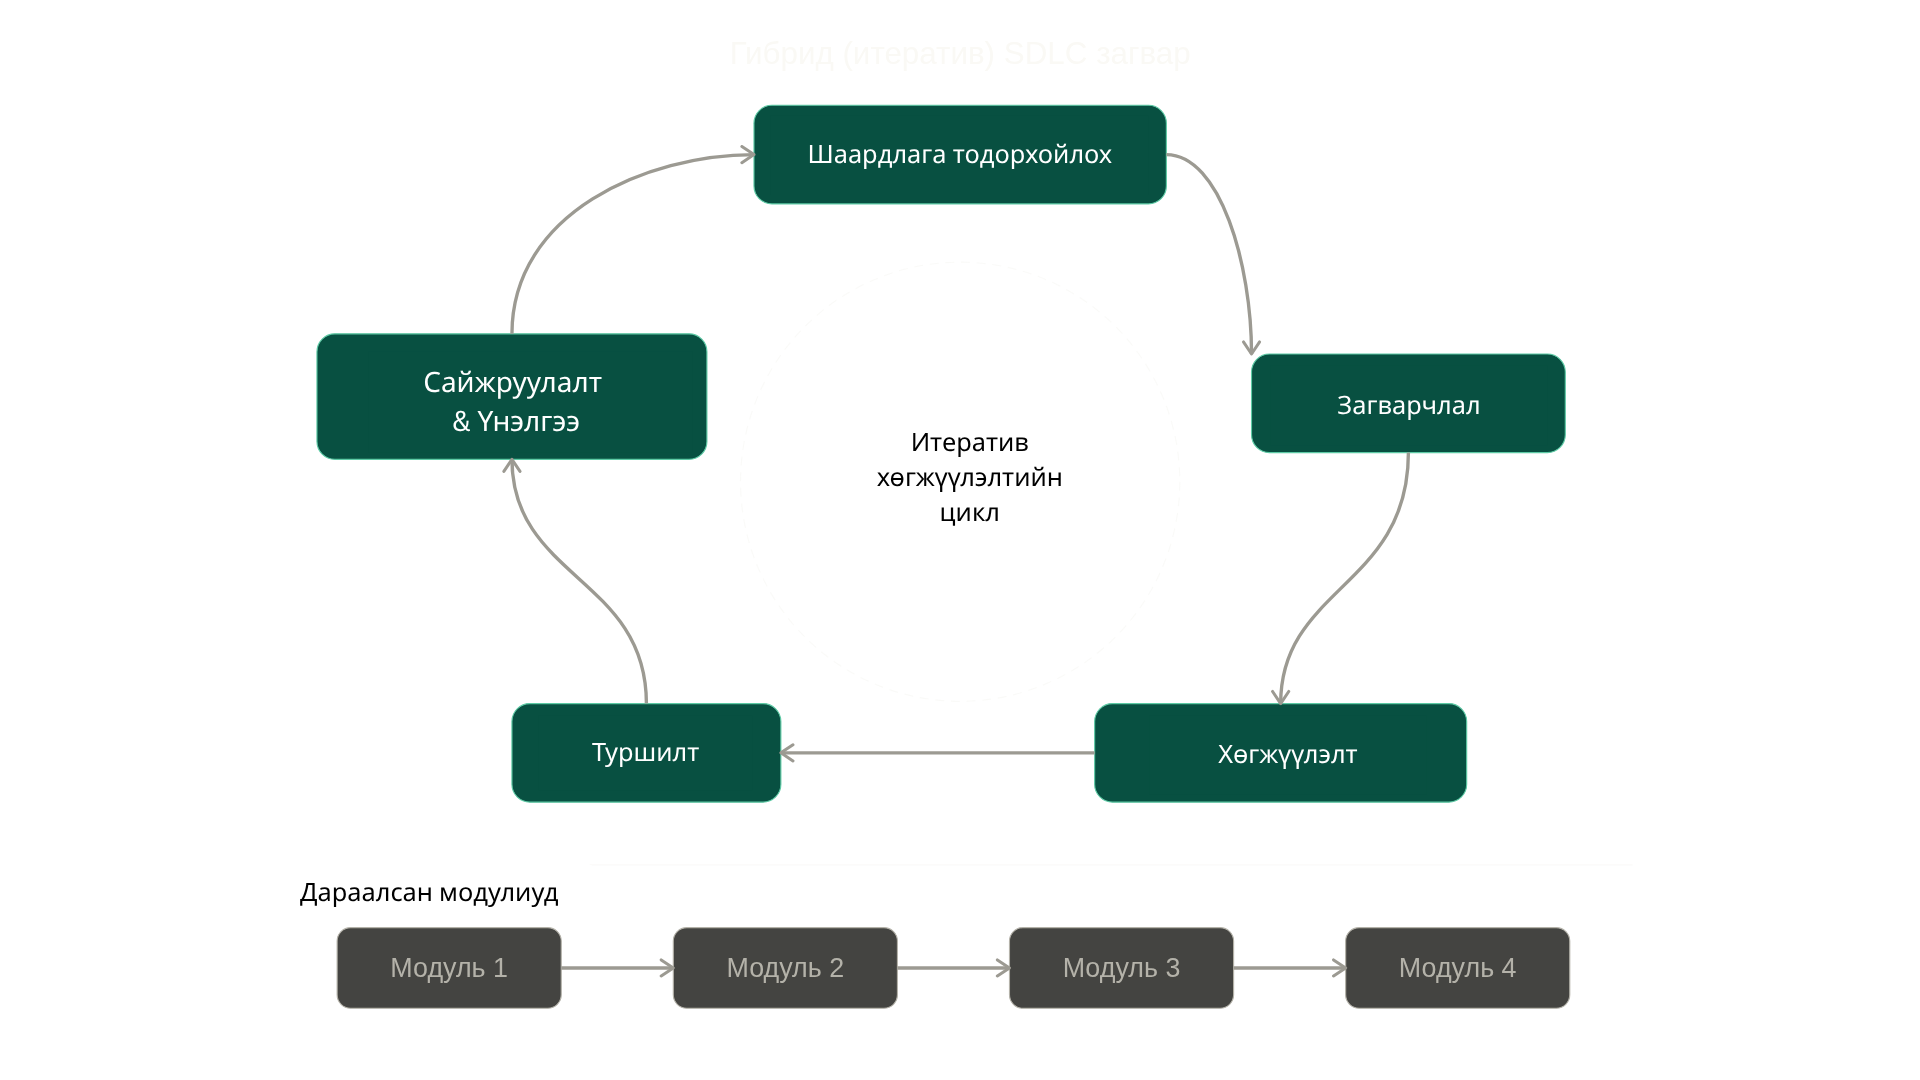
\includegraphics[width=0.92\textwidth]{pictures/hytbrid-iterative.png}
\caption{Итератив хөгжүүлэлтийн загварын ерөнхий схем}
\label{fig:hybrid-iterative-cycle}
\end{figure}




%==============================================================
\section{Системийн шинжилгээ ба шаардлага}
%==============================================================

\subsection{Одоо байгаа шийдлүүдийн харьцуулсан шинжилгээ}

Төстэй зургаан платформыг үндсэн таван функциональ үзүүлэлтээр харьцуулан шинжилсэн дүнг Хүснэгт~\ref{tab:system-compare}-д үзүүлэв.

\begin{table}[H]
\centering
\caption{Төстэй системүүдийн функциональ харьцуулалт}
\label{tab:system-compare}
\begin{tabular}{|p{2.6cm}|c|c|c|c|c|p{3.3cm}|}
\hline
\textbf{Систем} & \textbf{SRS} & \textbf{Толь} & \textbf{Хамтын орчин} & \textbf{Ранкинг} & \textbf{OCR} & \textbf{Гол онцлог} \\ \hline
Anki & Тийм & Үгүй & Үгүй & Үгүй & Үгүй & Гүнзгий давталтын алгоритм \\ \hline
Quizlet & Хэсэгчлэн & Үгүй & Тийм & Хэсэгчлэн & Үгүй & Флашкарт ба тоглоомчлол \\ \hline
Coursera & Үгүй & Үгүй & Хэсэгчлэн & Хэсэгчлэн & Үгүй & Бүтэцтэй онлайн сургалт \\ \hline
Stack Overflow & Үгүй & Үгүй & Тийм & Тийм & Үгүй & Q\&A ба reputation тогтолцоо \\ \hline
LeetCode & Үгүй & Үгүй & Хэсэгчлэн & Тийм & Үгүй & Алгоритмын сорилт, тэмцээн \\ \hline
\textbf{FutureHub} & Тийм & Тийм & Тийм & Тийм & Тийм & Суралцах, хамтын мэдлэг, ахицын нэгдсэн орчин \\ \hline
\end{tabular}
\end{table}

Хүснэгт~\ref{tab:system-compare}-аас харахад одоо зах зээл дээр байгаа платформуудын аль нь ч \textit{SRS, толь бичиг, хамтын орчин, ранкинг, OCR} гэсэн таван чиглэлийг нэгэн зэрэг шийдсэн шийдэл санал болгож чадахгүй байна. FutureHub нь тус бүр нь өөр өөр хэрэглэгчийн хэрэгцээг хангадаг эдгээр функцийг нэг бүтээгдэхүүн дотор нэгтгэж, өгөгдлийн нэгдсэн цөм дээр тулгуурлан ажиллуулахаар зохион байгуулагдсан.

\begin{figure}[htbp]
\centering
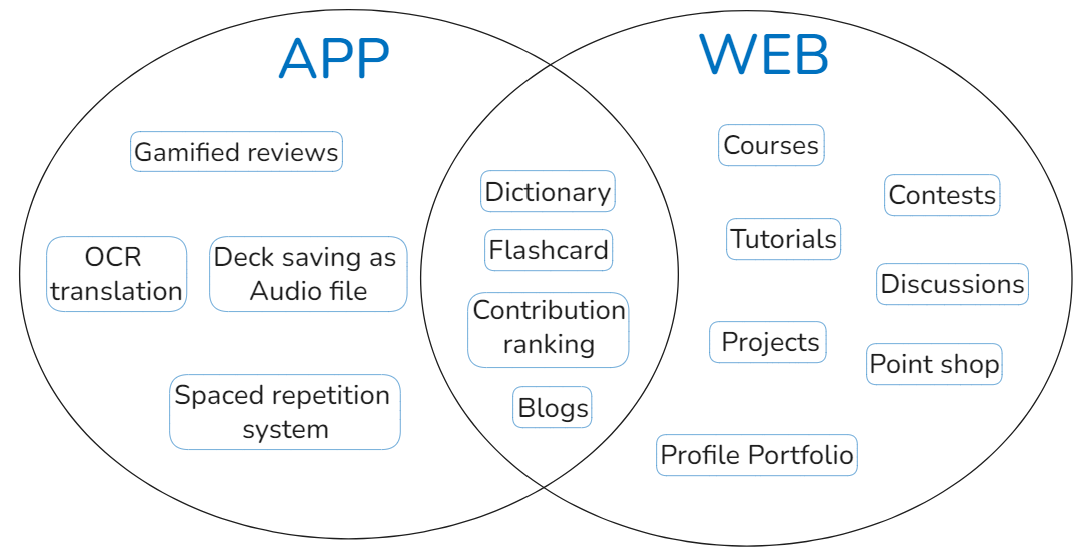
\includegraphics[width=0.9\textwidth]{pictures/functions-diagram.png}
\caption{Мобайл ба веб клиентүүдийн функцуудын огтлолцол}
\label{fig:function-venn}
\end{figure}

Зураг~\ref{fig:function-venn}-т FutureHub-ийн ``\textit{мобайл нь давталтын төвтэй, веб нь контентын төвтэй, хоёр талдаа нийтлэг өгөгдлийн цөмтэй}'' гэсэн зарчмыг үзүүлэв. Энэ нь хэрэглэгчийг нэг платформд хязгаарлахгүй, харин өдөр тутмын нөхцөл байдалдаа тохирсон орчноос үргэлжлүүлэн суралцах уян хатан байдлыг олгоно. Иймээс FutureHub-ийн судалгааны үнэ цэн нь ``\textit{аль нэг модулийг сайжруулах}'' бус, харин \textbf{суралцах үйл явцыг бүхэлд нь дэмжих интеграцчилсан орчин} бий болгоход оршино.

\subsection{Функциональ шаардлага}

Функциональ шаардлагыг ач холбогдлын түвшингээр ялган \textit{Core} (үндсэн) ба \textit{Extended} (өргөтгөсөн) гэсэн хоёр ангилалд тодорхойлов.

\subsubsection{Core шаардлага}

\begin{itemize}
    \item Хэрэглэгчийн бүртгэл, нэвтрэлт, эрхийн удирдлага
    \item Хэрэглэгчийн профайл, тохиргоо, нотификацийн систем
    \item Толь бичигт нэр томьёо хайх, нэмэх, тайлбарлах
    \item Q\&A асуулт асуух, хариулт өгөх, санал хураах
    \item Нийтлэл бичих, орчуулах
    \item Ranking тооцох, үзүүлэх
    \item Бүтээлээ хуваалцах, бусдын бүтээлд сэтгэгдэл үлдээх
\end{itemize}
    

\subsubsection{Extended шаардлага}

\begin{itemize}
    \item Тэмцээн зохион байгуулах, хугацаа ба оролцоог хянах
    \item SRS-д суурилсан флашкарт үүсгэх, засах, давтах
    \item Хэрэглэгчийн ахиц, идэвхжилийн аналитик үзүүлэлт гаргах
    \item OCR ашиглан зурагнаас текст таних, флашкарт үүсгэх
    \item Оноо цуглуулан дэлгүүрээс бараа авах
    \item Сургалтын нэмэх, удирдах, оюутанд зөвлөмж өгөх
\end{itemize}

\subsubsection{Хэрэглэгчийн эрхээр ангилсан шаардлагын матриц}

\begin{table}[H]
\centering
\caption{Хэрэглэгчийн эрхээр ангилсан функциональ шаардлагын матриц}
\label{tab:role-requirements}
\begin{tabular}{|c|c|c|c|}
\hline
\textbf{Шаардлага} & \textbf{Оюутан} & \textbf{Багш} & \textbf{Админ} \\ \hline
Флашкарт үүсгэх, давтах & \checkmark & \checkmark & -- \\ \hline
Толь бичиг хайх, нэмэх & \checkmark & \checkmark & -- \\ \hline
Q\&A асуулт/хариулт & \checkmark & \checkmark & -- \\ \hline
Нийтлэл бичих, орчуулах & \checkmark & \checkmark & -- \\ \hline
Бүтээл хуваалцах & \checkmark & \checkmark & -- \\ \hline
Сургалт, тэмцээн удирдах & -- & \checkmark & \checkmark \\ \hline
Контент баталгаажуулах & -- & \checkmark & \checkmark \\ \hline
Хэрэглэгчийн эрх удирдах & -- & -- & \checkmark \\ \hline

\end{tabular}
\end{table}

\subsection{Функциональ бус шаардлага ба хязгаарлалт}

\begin{itemize}
    \item \textbf{Гүйцэтгэл:} гол хүсэлтүүдийг бодит хэрэглээнд саатал багатайгаар боловсруулах (API-ийн дундаж хариу өгөх хугацаа 500 мс-ээс бага байх)
    \item \textbf{Аюулгүй байдал:} JWT-д суурилсан нэвтрэлт, RBAC-ийн үүргийн зөвшөөрөл,PostgreSQL RLS бодлогоор мөрийн түвшний хамгаалалтыг хослуулан хэрэгжүүлэх
    \item \textbf{Өргөтгөх боломж:} шинэ модуль нэмэхэд өгөгдлийн загварын суурь бүтцийг эвдэхгүй байхаар зохион байгуулах
    \item \textbf{Найдвартай байдал:} өгөгдлийн нөөцлөлт ба сэргээх боломж, алдааны бүртгэлийн дэмжлэг
    \item \textbf{Хязгаарлалт:} сургуулийн албан ёсны бүртгэлтэй хэрэглэгчдэд чиглэсэн хандалтын бодлого баримтлах
\end{itemize}

\subsection{Бизнес процессын загварчлал (UML)}

\subsubsection{Контекст диаграм}

Системд оролцогч гурван үүрэг бүр нь өөрийн онцлогт тохирсон үйлдлийн багцтай:
\begin{itemize}
    \item \textbf{Оюутан:} флашкарт үүсгэх, толь бичигт нэр томьёо нэмэх, асуулт асуух, нийтлэл бичих, бусдын бүтээлд сэтгэгдэл үлдээх
    \item \textbf{Багш:} сургалт удирдах, тэмцээн зохион байгуулах, контент баталгаажуулах
    \item \textbf{Админ:} хэрэглэгчийн эрх удирдах, системийн тохиргоо хийх
\end{itemize}
\begin{figure}[htbp]
\centering
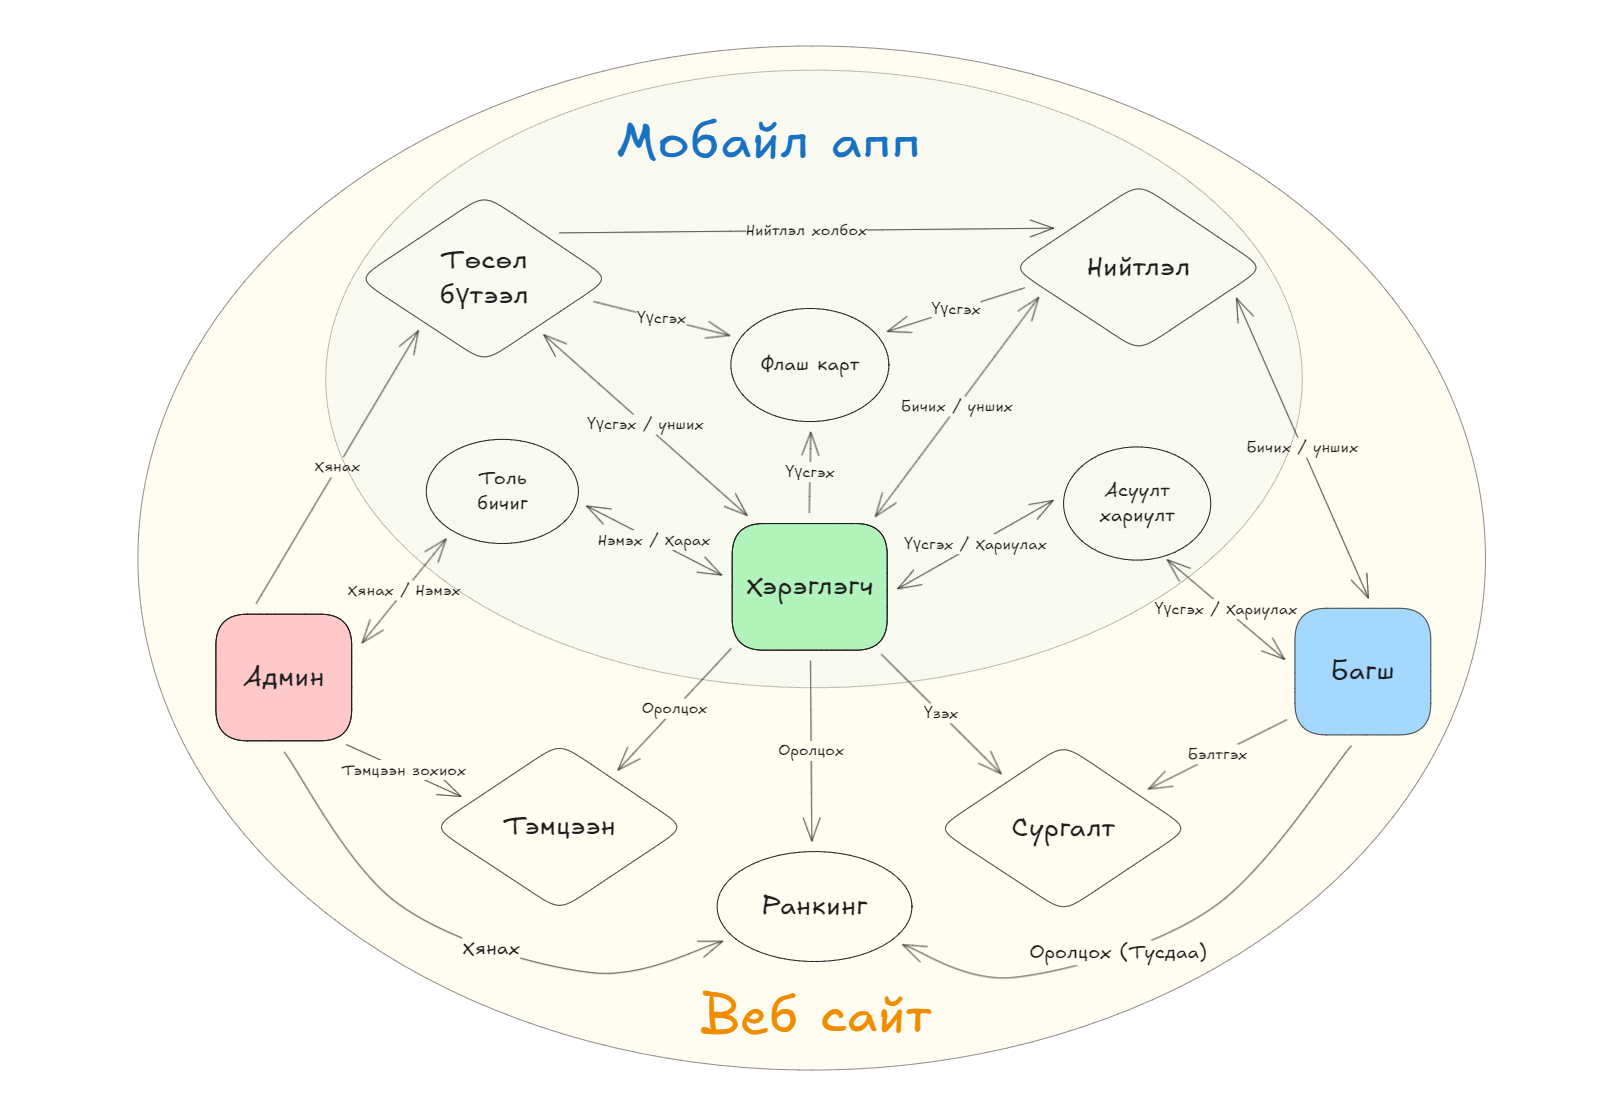
\includegraphics[width=0.92\textwidth]{pictures/futurehub-context.png}
\caption{FutureHub системийн контекст диаграм}
\label{fig:futurehub-context}
\end{figure}

\subsubsection{Sequence диаграмууд}

Системийн үндсэн боловсруулалтууд болох Flashcard review, OCR based generation, article dicitonary creationз зэргийг Sequence диаграмаар загварчилж харуулав. Зураг~\ref{fig:futurehub-sequence-overview}-д системийн ерөнхий урсгалыг, Зураг~\ref{fig:futurehub-seq-auth}--\ref{fig:futurehub-seq-contest}-т тус бүрийн нарийвчилсан урсгалыг үзүүлэв.

\begin{figure}[htbp]
\centering
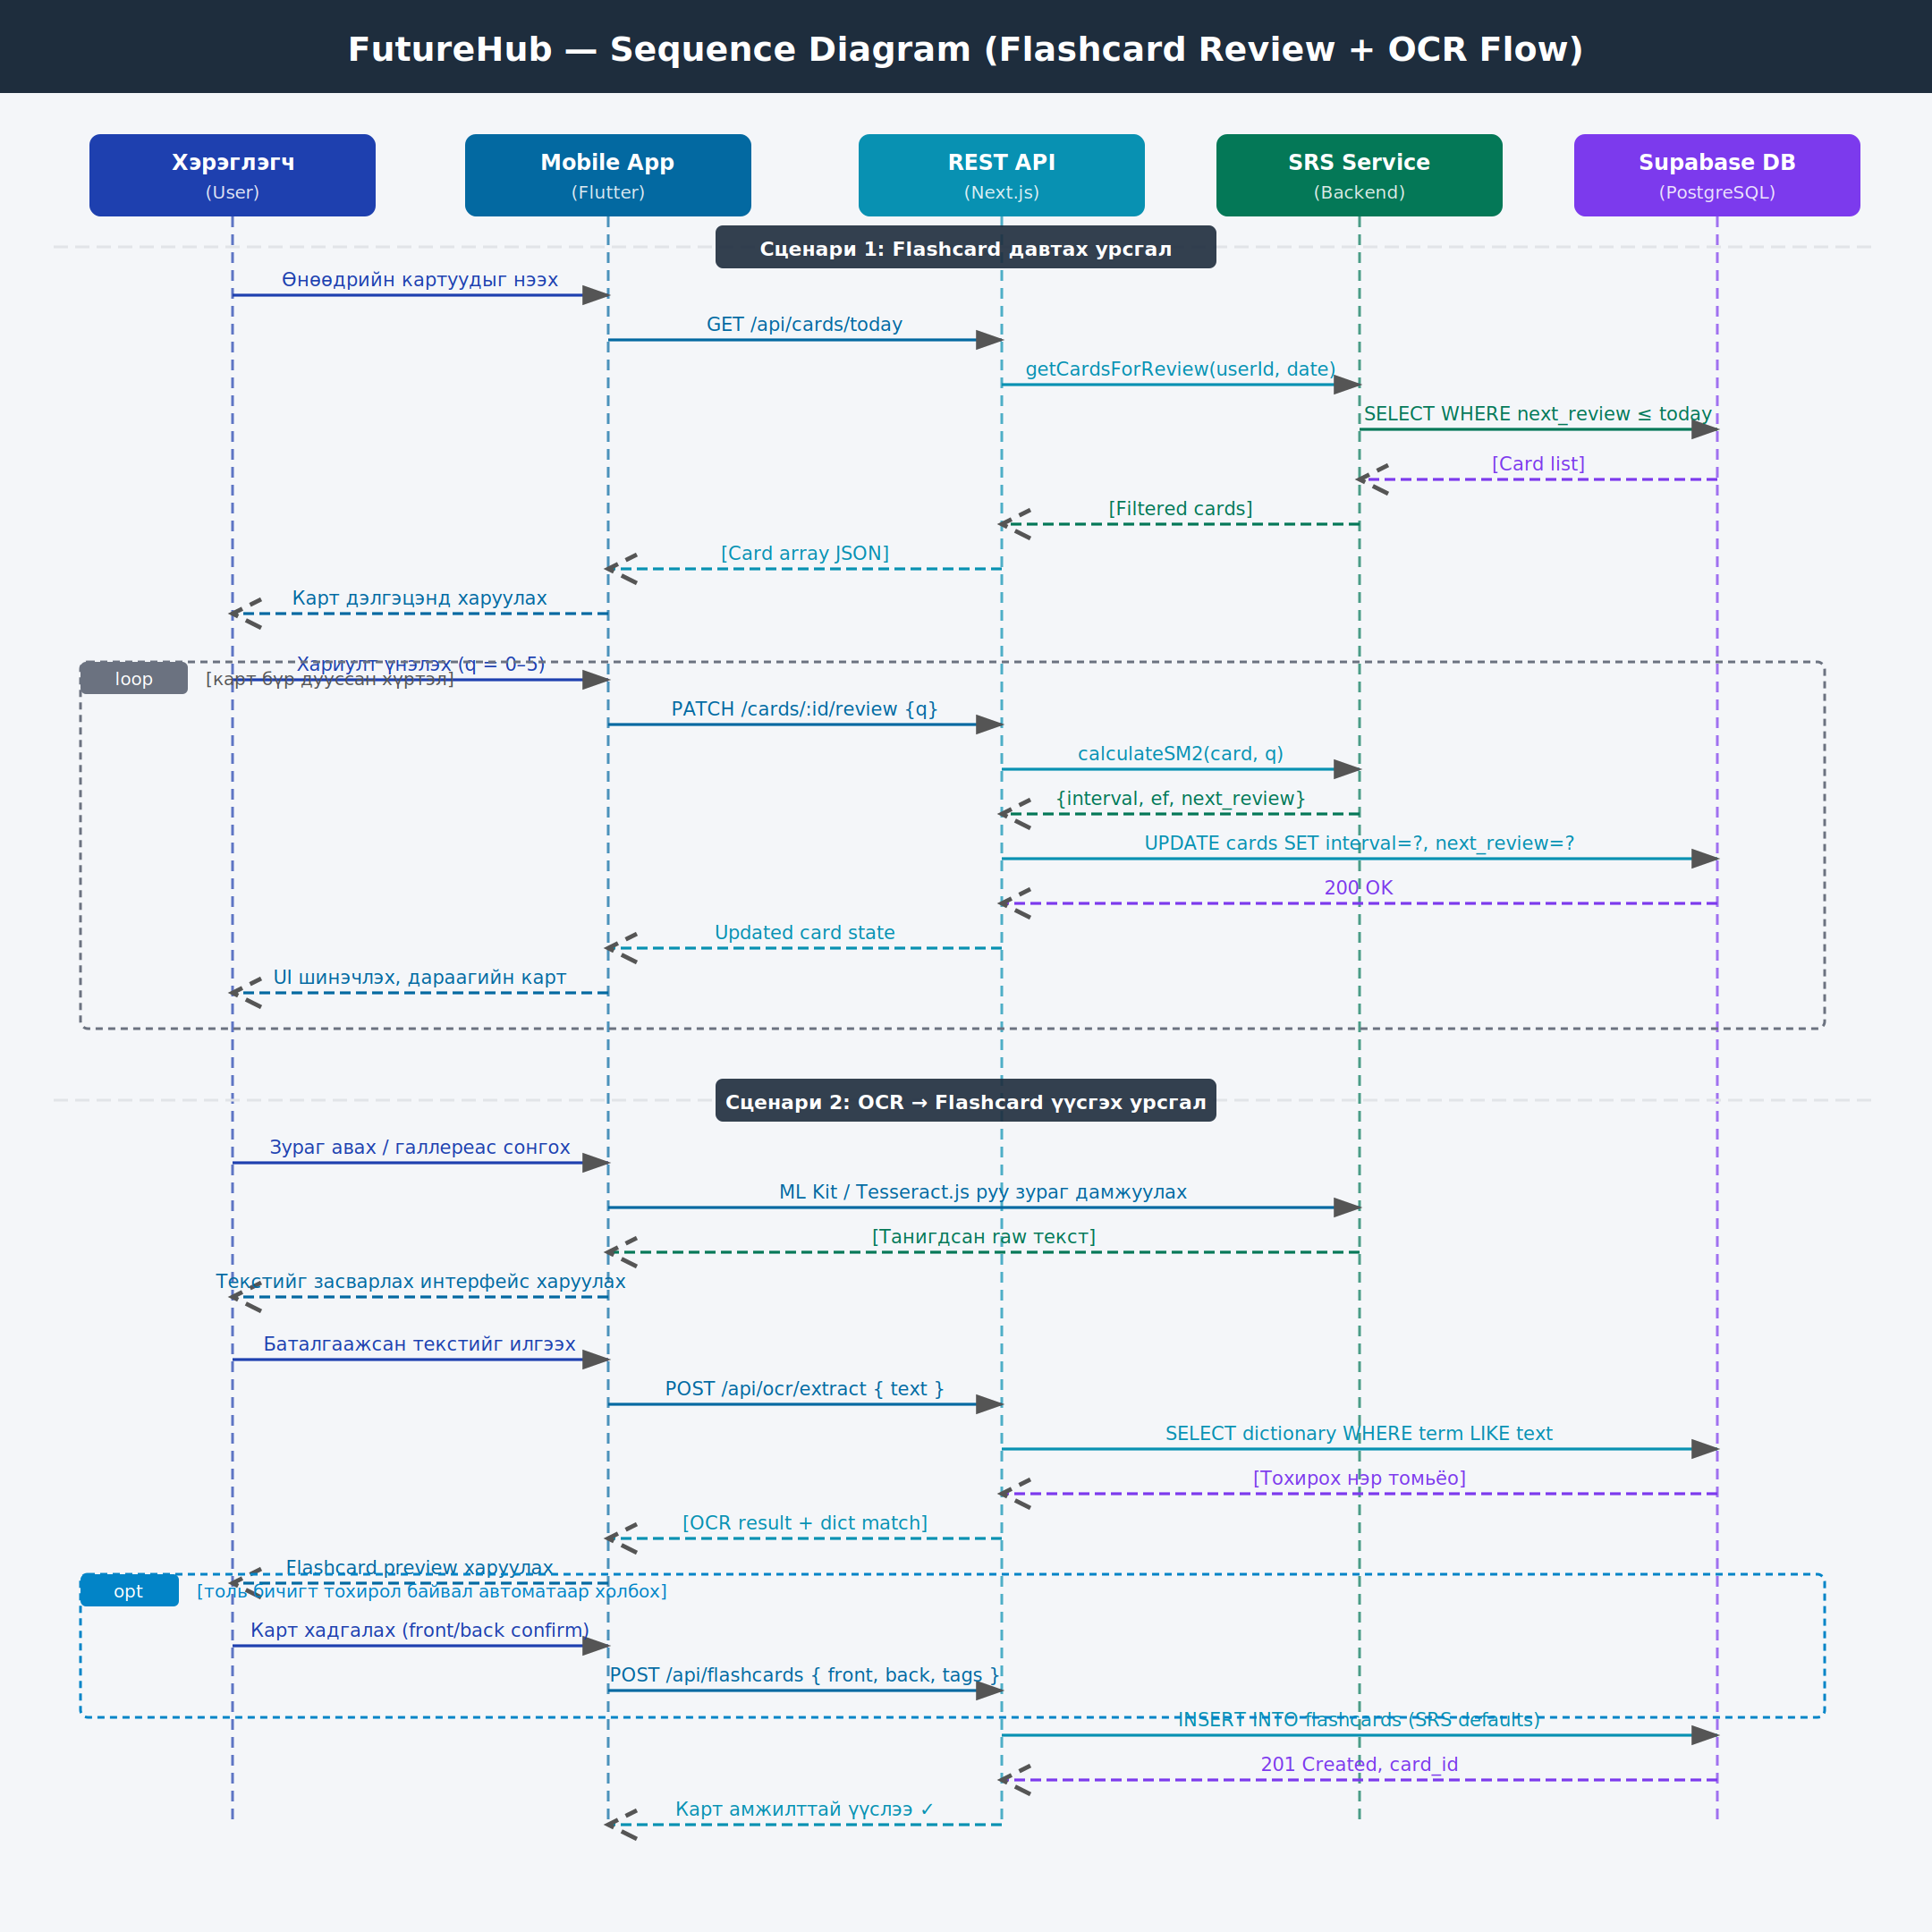
\includegraphics[width=0.92\textwidth]{pictures/futurehub_3_sequence.png}
\caption{FutureHub Flashcard review +  OCR flow диаграм}
\label{fig:futurehub-sequence-overview}
\end{figure}


\begin{figure}[htbp]
\centering
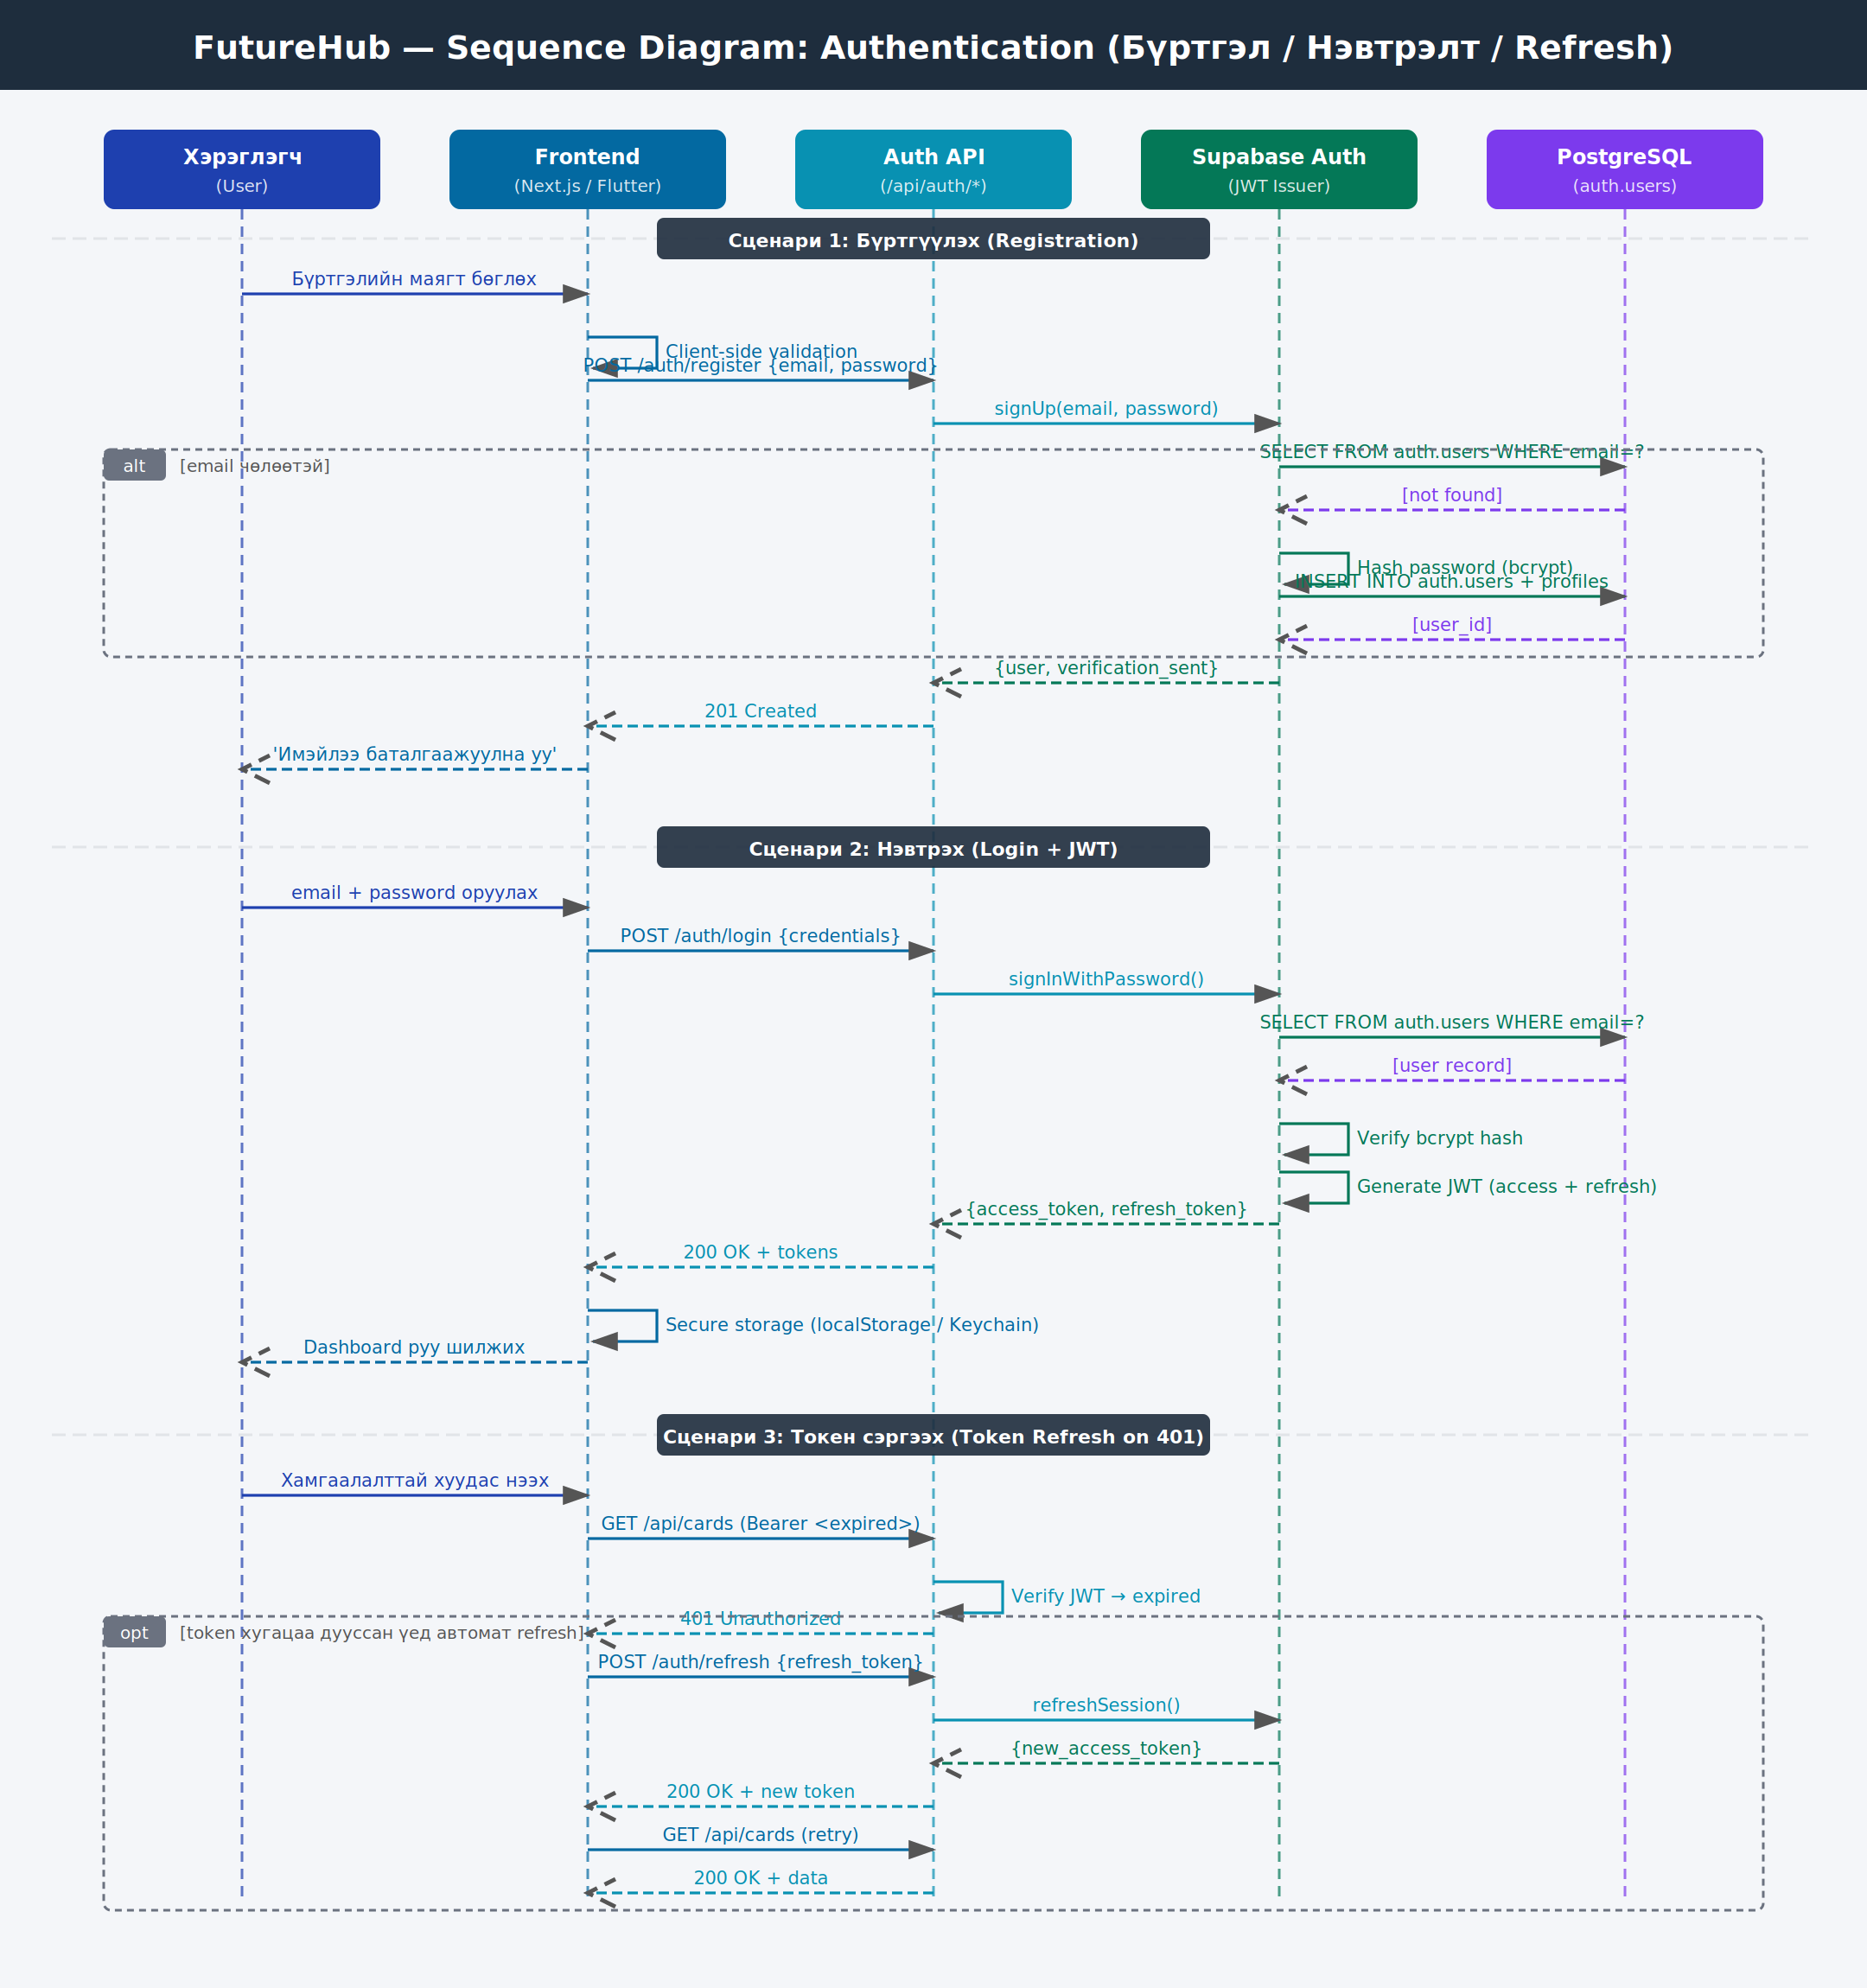
\includegraphics[width=0.92\textwidth]{pictures/futurehub_seq_auth.png}
\caption{Нэвтрэлт ба зөвшөөрлийн урсгалын Sequence диаграм}
\label{fig:futurehub-seq-auth}
\end{figure}


\begin{figure}[htbp]
\centering
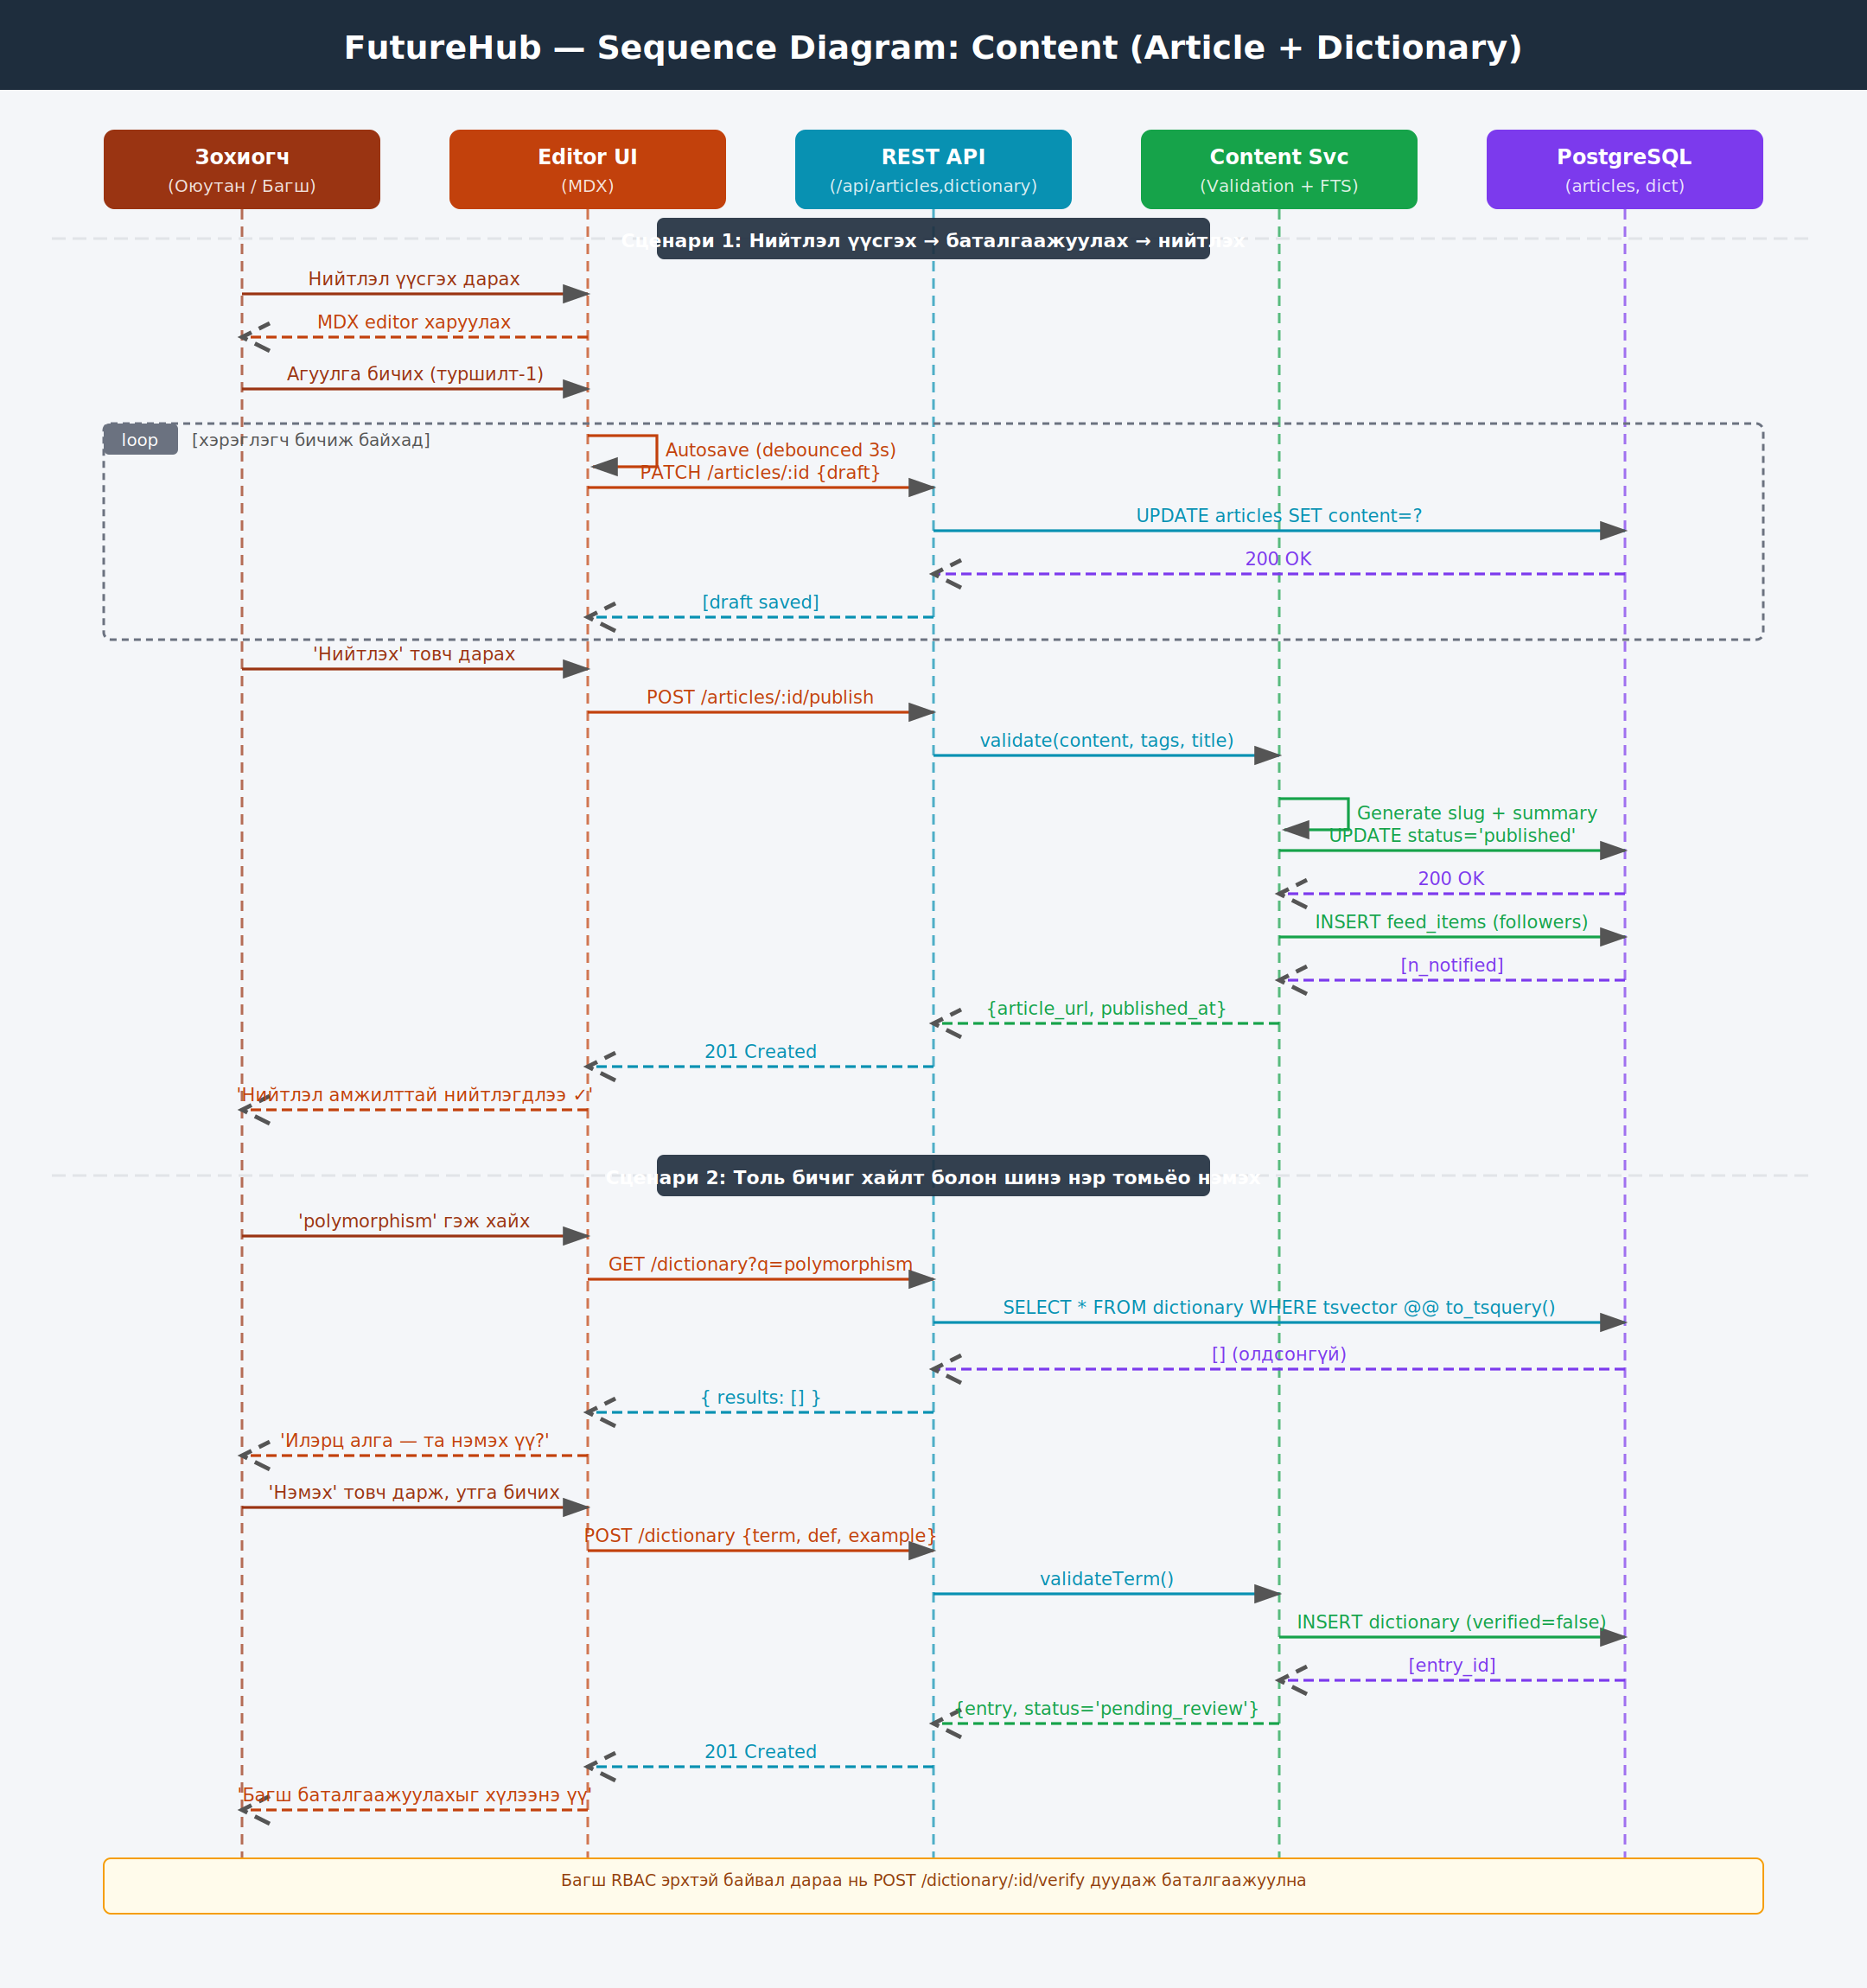
\includegraphics[width=0.92\textwidth]{pictures/futurehub_seq_content.png}
\caption{Контент үүсгэх урсгалын Sequence диаграм}
\label{fig:futurehub-seq-content}
\end{figure}

\begin{figure}[htbp]
\centering
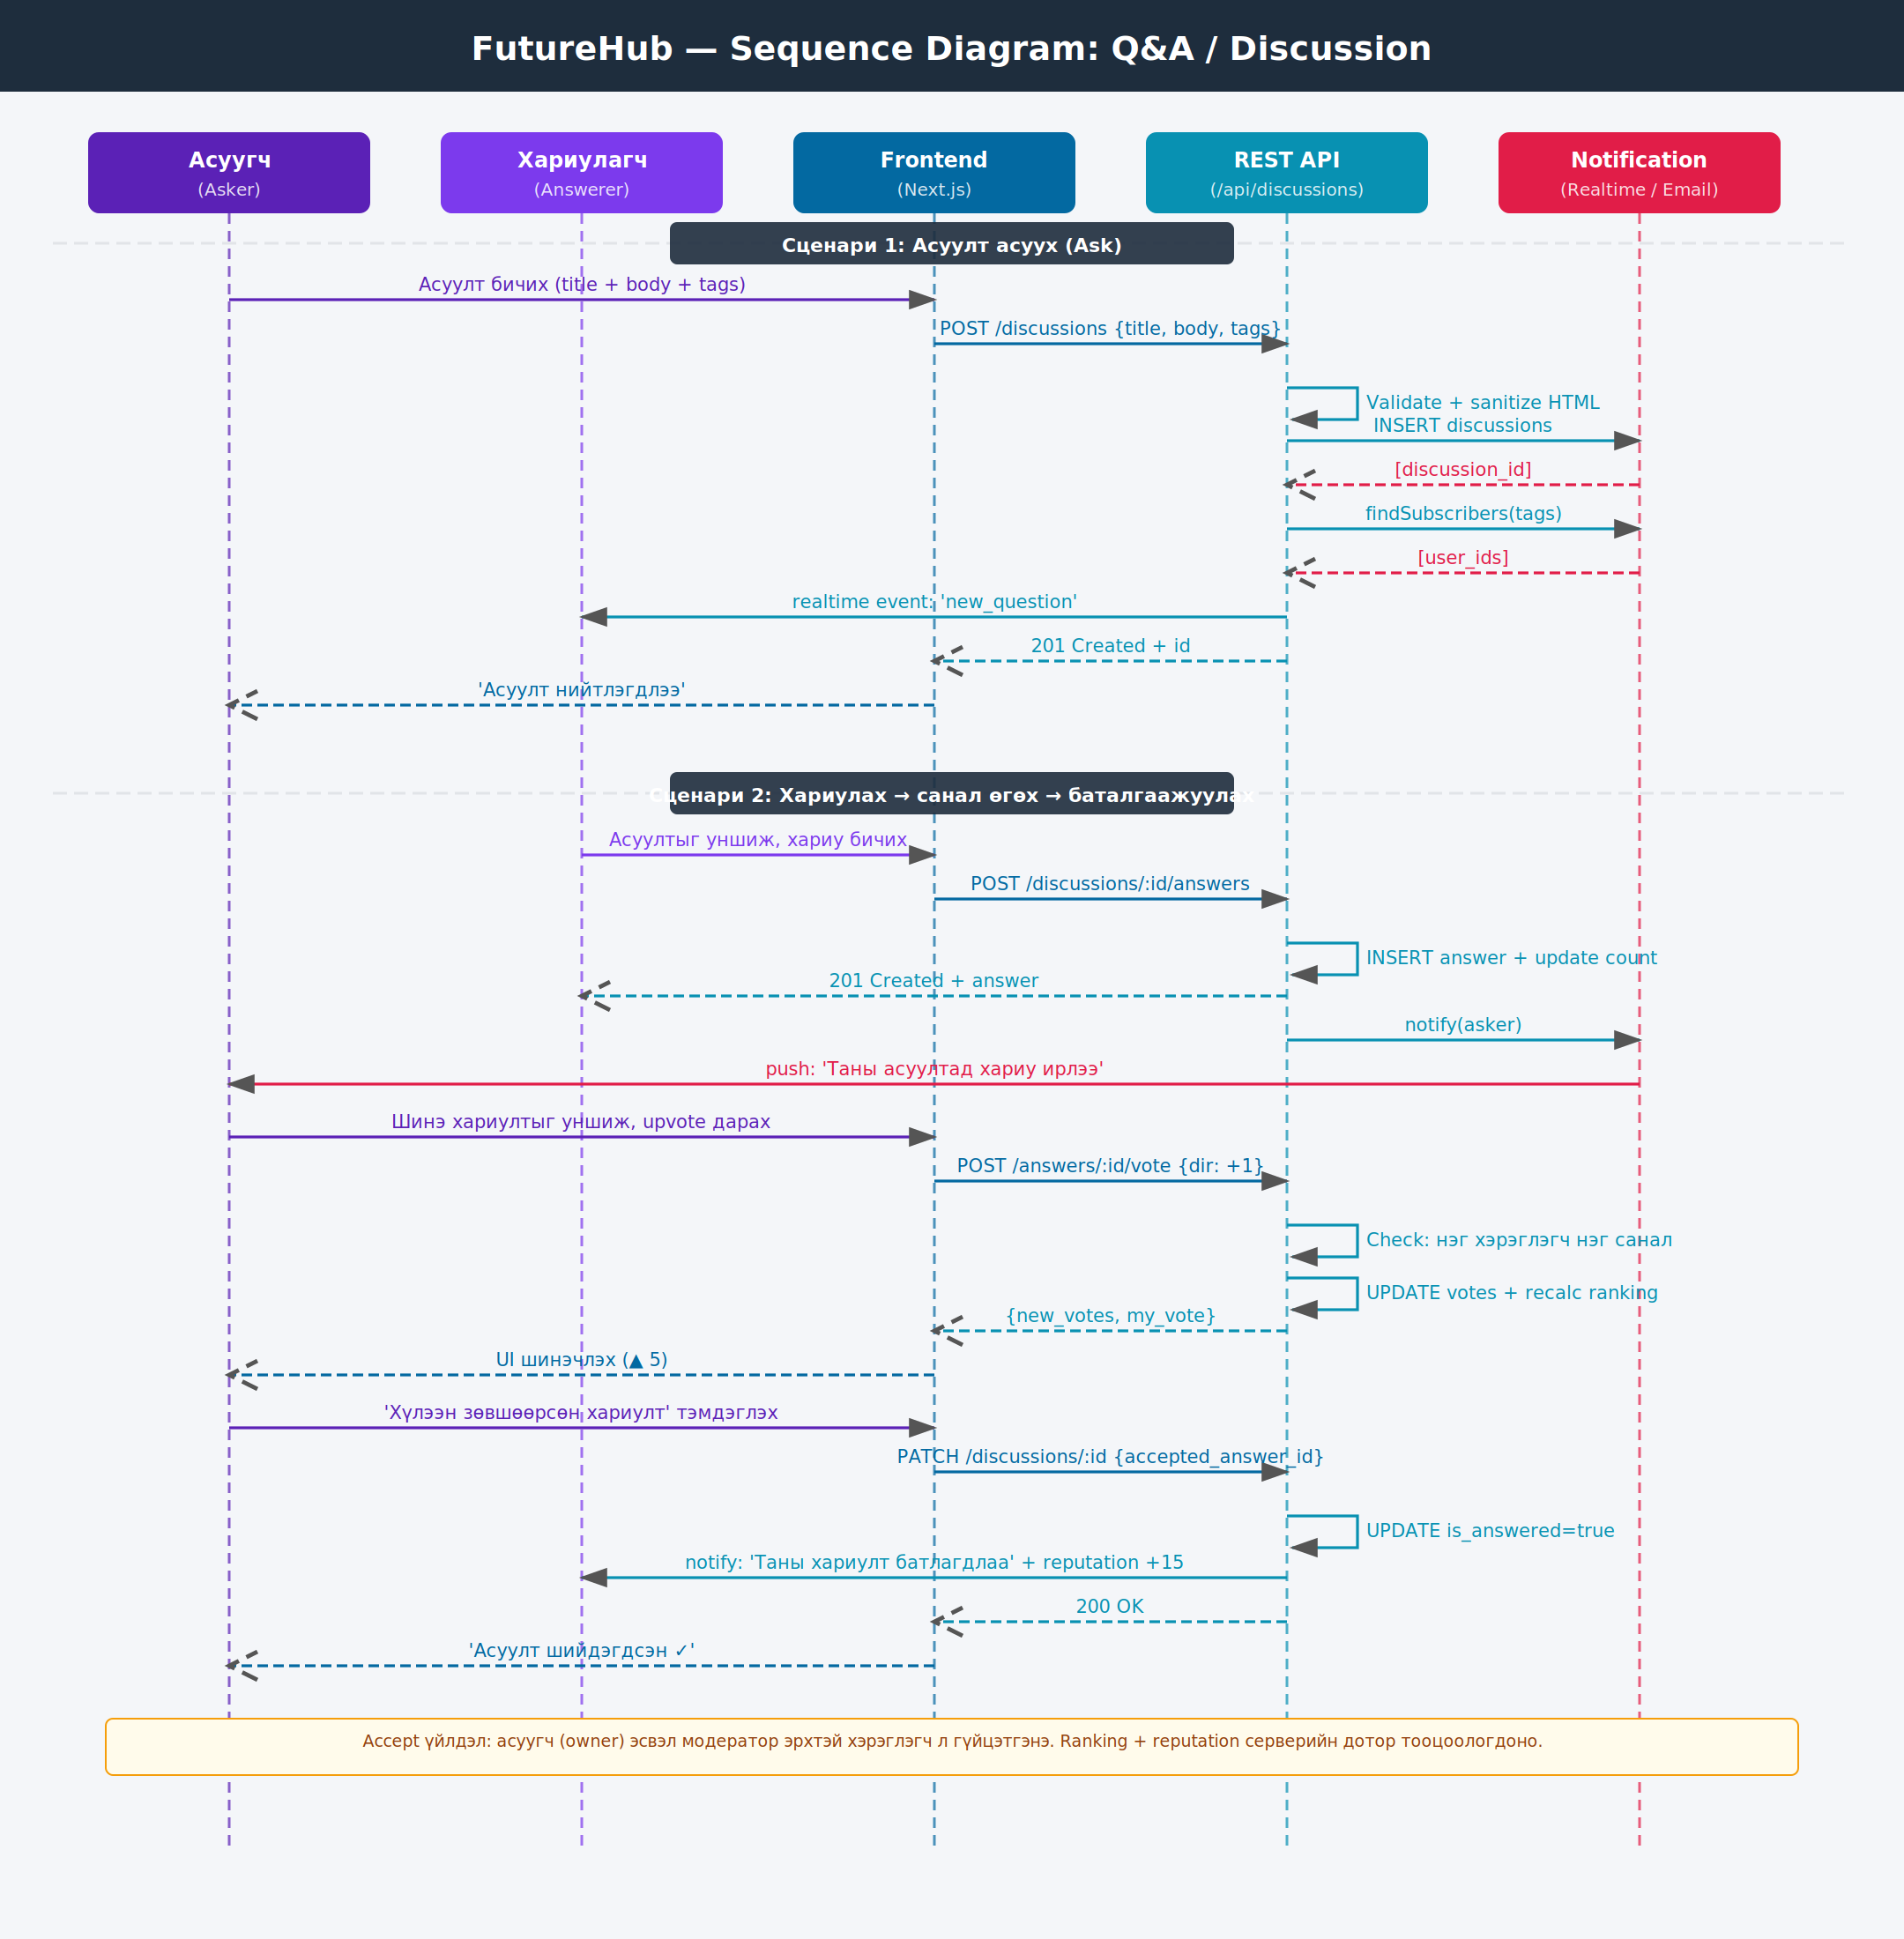
\includegraphics[width=0.92\textwidth]{pictures/futurehub_seq_qa.png}
\caption{Q\&A урсгалын Sequence диаграм}
\label{fig:futurehub-seq-qa}
\end{figure}

\begin{figure}[htbp]
\centering
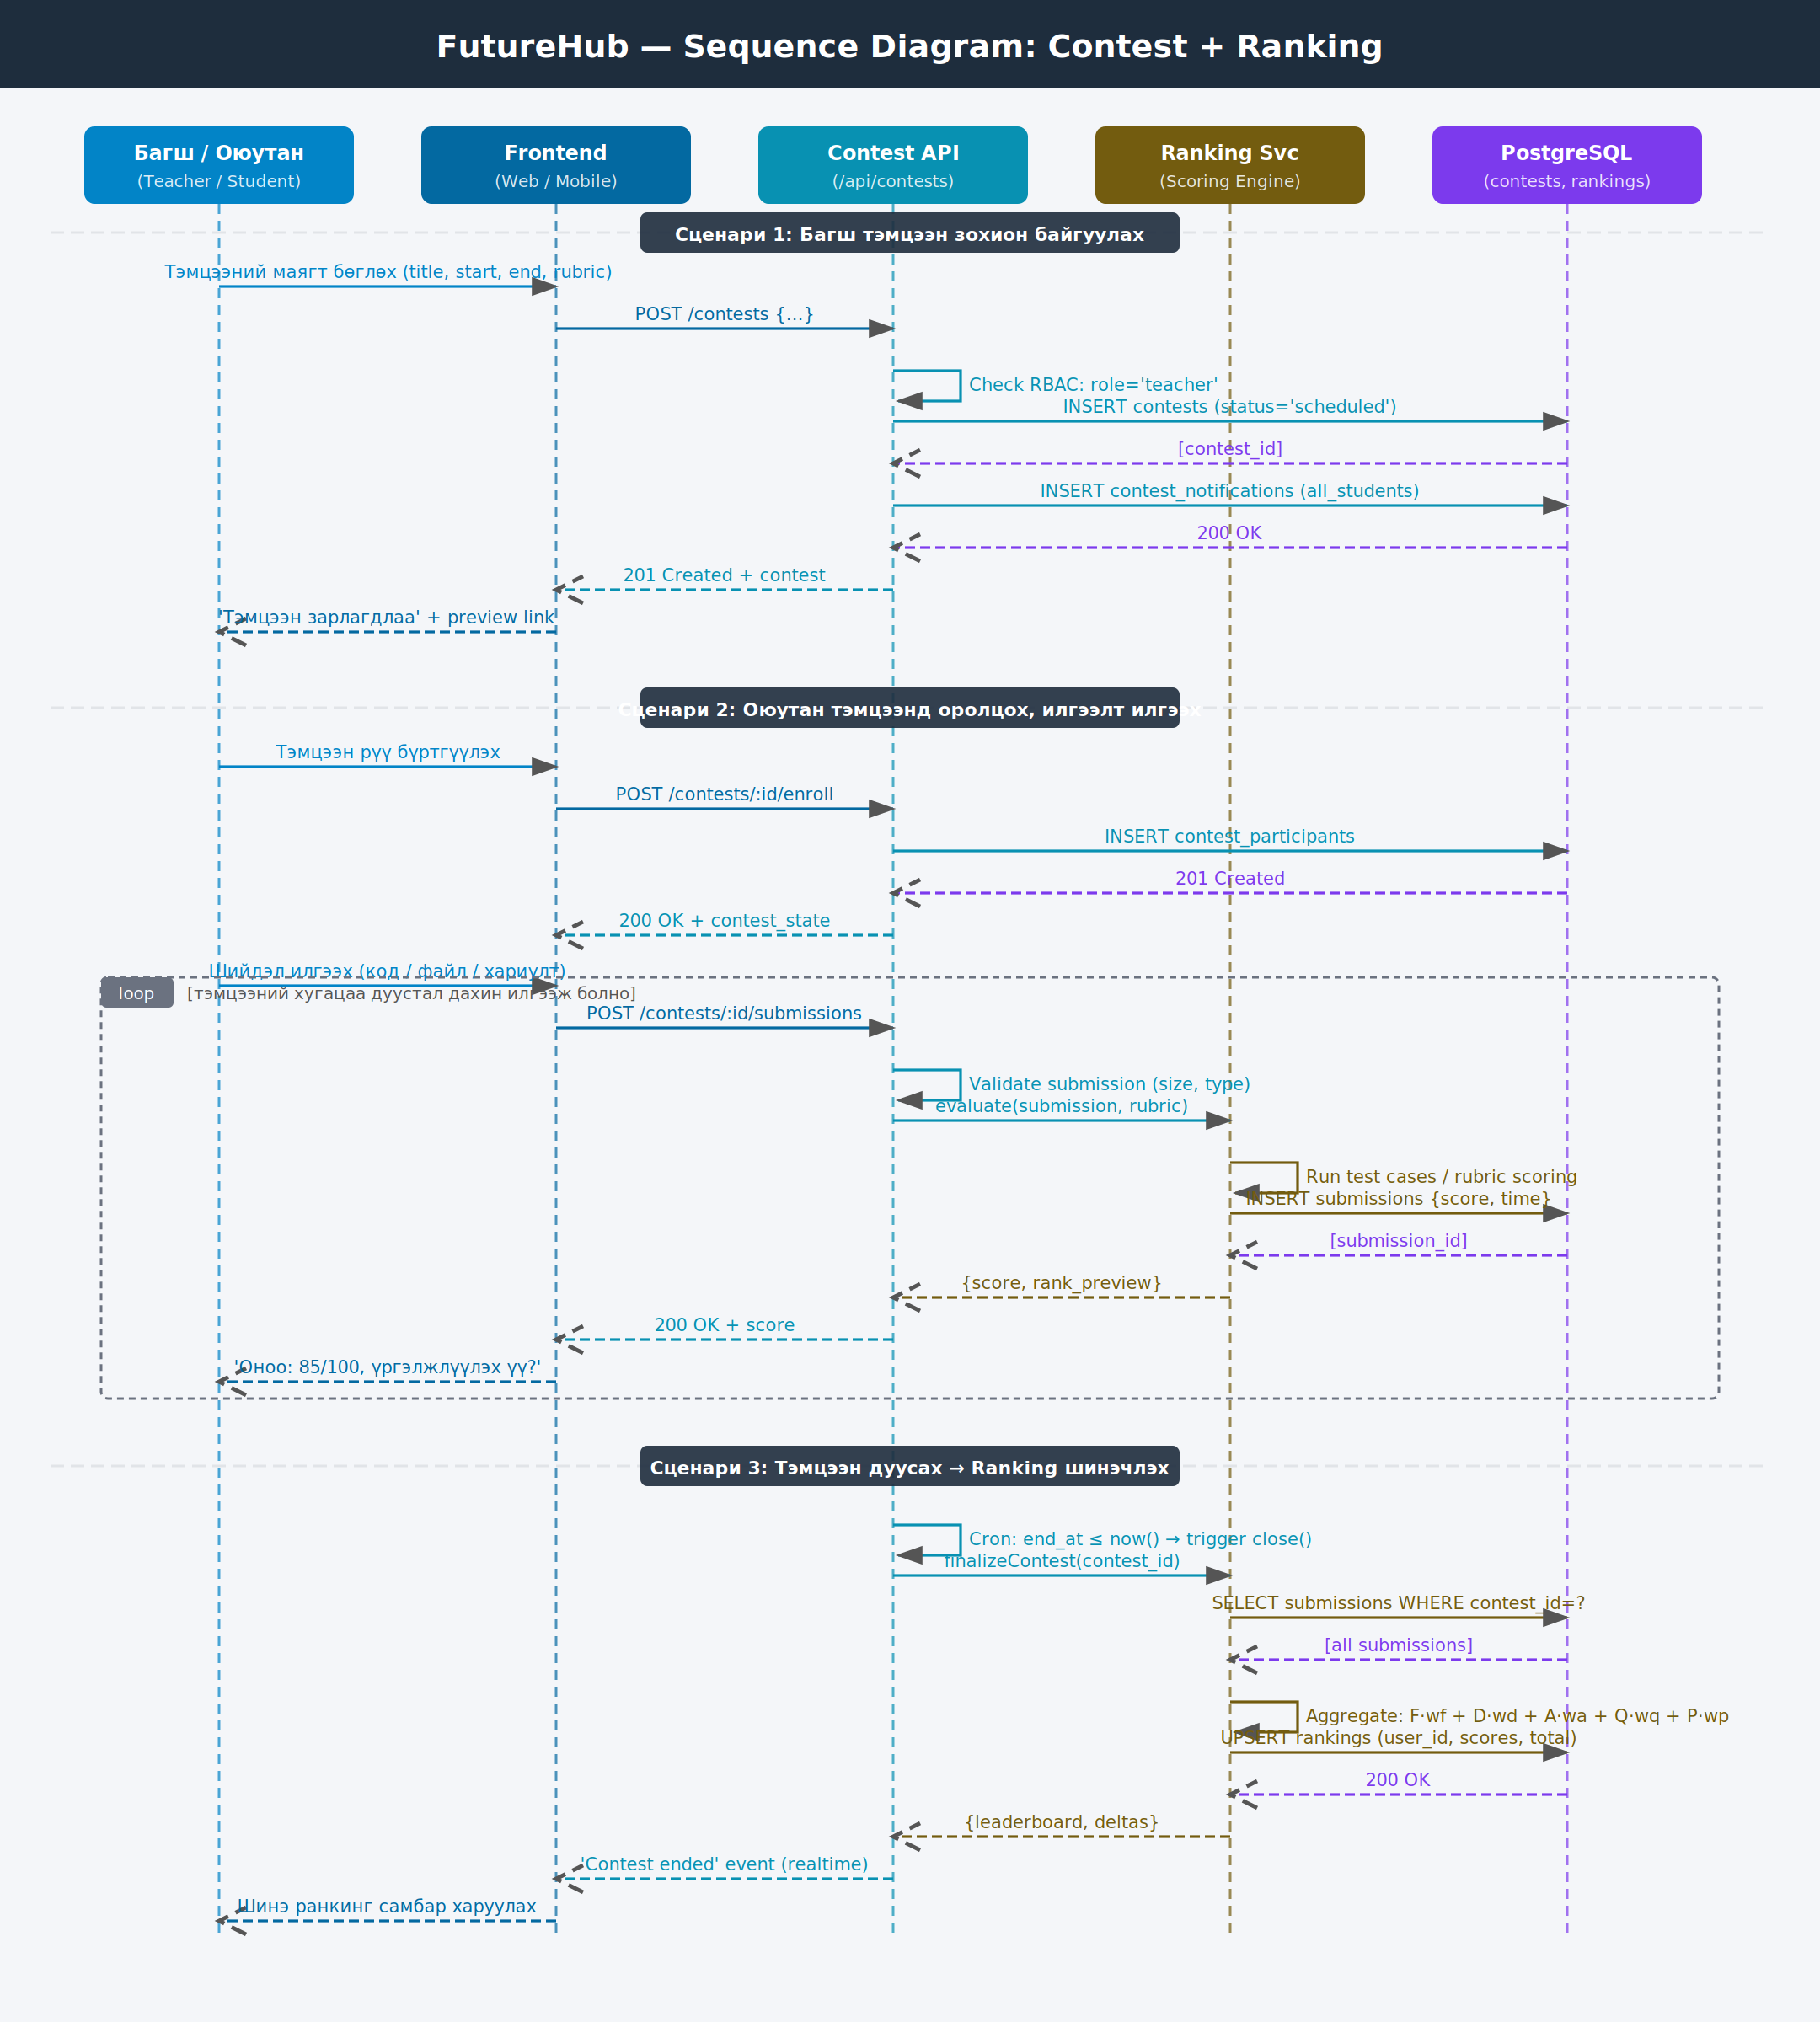
\includegraphics[width=0.92\textwidth]{pictures/futurehub_seq_contest.png}
\caption{Тэмцээний урсгалын Sequence диаграм}
\label{fig:futurehub-seq-contest}
\end{figure}

%==============================================================
\section{Системийн архитектур ба технологийн шийдэл}
%==============================================================

\subsection{Архитектурын дизайн}

Системийг \textbf{Web (Vercel)}, \textbf{Mobile (Flutter)}, \textbf{Backend (Supabase)} гэсэн гурван байршуулалтын (deployment) түвшинд зохион байгуулсан. Клиент хэсгүүд нь REST API-ийн нэгдсэн давхаргаар дамжин backend үйлчилгээтэй харилцах бөгөөд ингэснээр бизнес логикийн давхардлыг багасгаж, өөрчлөлтийг төвлөрсөн байдлаар удирдах боломжтой болно.

\begin{figure}[htbp]
\centering
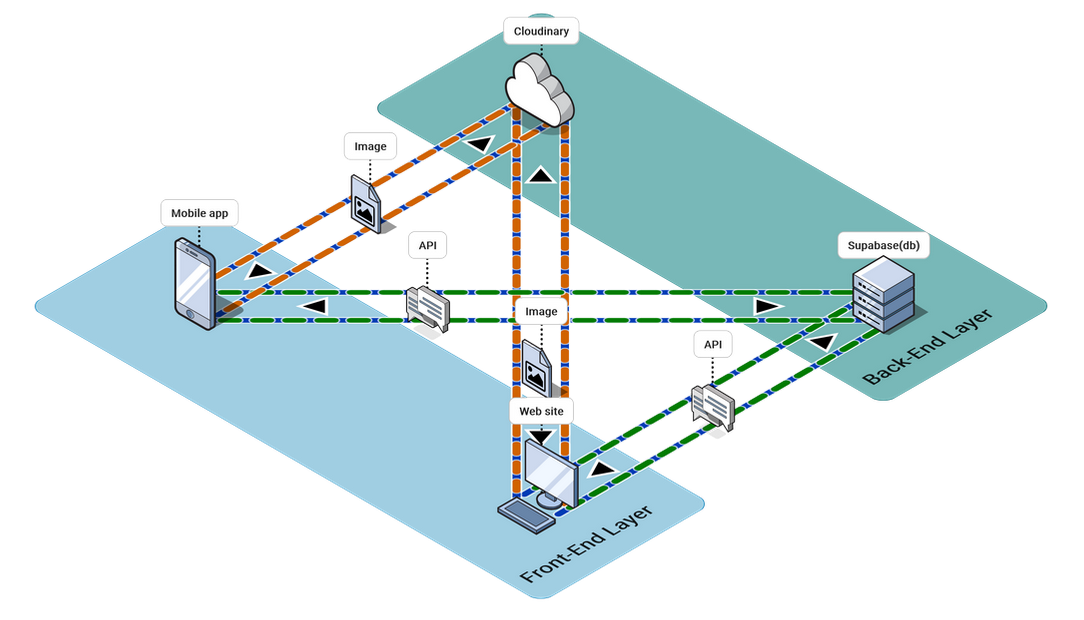
\includegraphics[width=0.98\textwidth]{pictures/system-architecture.png}
\caption{FutureHub системийн архитектурын зураглал}
\label{fig:system-architecture}
\end{figure}

\subsubsection{Аюулгүй байдал ба хандалтын хяналт}

Систем нь гурван түвшний хамгаалалтын загварыг хэрэгжүүлнэ:

\begin{itemize}
    \item \textbf{JWT (JSON Web Token):} хэрэглэгчийн нэвтрэлт ба сесс удирдлагыг stateless загвараар хангах
    \item \textbf{RBAC (Role-Based Access Control):} оюутан, багш, админ гэсэн үүрэг тус бүрт оноосон зөвшөөрлийн багц
    \item \textbf{RLS (Row-Level Security):} PostgreSQL-ийн мөрийн түвшинд өгөгдлийн хандалтыг хязгаарлах бодлого
\end{itemize}

Энэхүү давхар хамгаалалт нь аппликэйшн болон өгөгдлийн сангийн түвшинд аюулгүй байдлыг давхарлан баталгаажуулна.

\subsection{Технологийн стек ба сонголтын үндэслэл}

Технологи тус бүрийг \textit{шийдэж буй асуудалтай нь холбон} Хүснэгт~\ref{tab:tech-stack}-д нэгтгэн үзүүлэв.

\begin{table}[H]
\centering
\caption{Технологийн стек ба шийдэж буй асуудлын уялдаа}
\label{tab:tech-stack}
\begin{tabular}{|p{3.2cm}|p{3.4cm}|p{7cm}|}
\hline
\textbf{Давхарга} & \textbf{Технологи} & \textbf{Шийдэж буй асуудал ба үндэслэл} \\ \hline
Frontend (Web) & Next.js & SSR/SSG дэмжлэгтэй тул SEO ба эхний ачаалалтын хурдыг сайжруулж, өргөтгөх боломжтой \\ \hline
Frontend (Mobile) & Flutter & Нэг кодын баазаас Android, iOS руу нэгэн зэрэг хөгжүүлэх боломжтой, UI-ийн үзүүлэлт өндөр \\ \hline
Backend \& DB & Supabase (PostgreSQL) & Real-time DB, Auth, Storage-ийг нэг платформоос шийдсэнээр infra-ийн тархмал байдлыг багасгана \\ \hline
OCR & ML Kit (Mobile), Tesseract.js (Web) & Зургаас текст таних ажиллагааг хоёр платформд нутагшуулахад зориулсан сонголт \\ \hline
State management & React Context + Hooks, Riverpod & Модулийн түвшний төлвийн удирдлага, тест бичихэд тохиромжтой бүтэц \\ \hline
Version control & Git / GitHub & Итераци бүрийн өөрчлөлтийг бүртгэх, хамтын хөгжүүлэлтийн workflow-г дэмжих \\ \hline
\end{tabular}
\end{table}

\subsection{Өгөгдлийн сангийн зохиомж}

\textbf{ER түвшний үндсэн entity-үүд:} \texttt{users}, \texttt{flashcards}, \texttt{dictionary\_entries}, \texttt{articles}, \texttt{discussions}, \texttt{project\_logs}, \texttt{contests}, \texttt{rankings}.

Гол зохион байгуулалтын зарчмууд:

\begin{itemize}
    \item \textbf{Харилцан хамаарал:} хэрэглэгч--агуулга (1\,:\,n), флашкарт--толь бичиг (n\,:\,n), тэмцээн--оролцогч (n\,:\,n) гэх зэрэг холбоосуудыг normalize хэлбэрээр зохион байгуулсан
    \item \textbf{Индексжүүлэлт:} full-text хайлтын \texttt{GIN} индекс, давталтын шалгалтад \texttt{next\_review}-ийн индекс, ранкингийн \texttt{score} талбарын индексийг тус тус үүсгэсэн
    \item \textbf{Бодлогын түвшин:} PostgreSQL RLS ашиглан хэрэглэгч зөвхөн өөрийн зөвшөөрөгдсөн мөрүүдийг харах, өөрчлөх боломжтой байхаар тохируулсан
\end{itemize}

\begin{figure}[H]
\centering
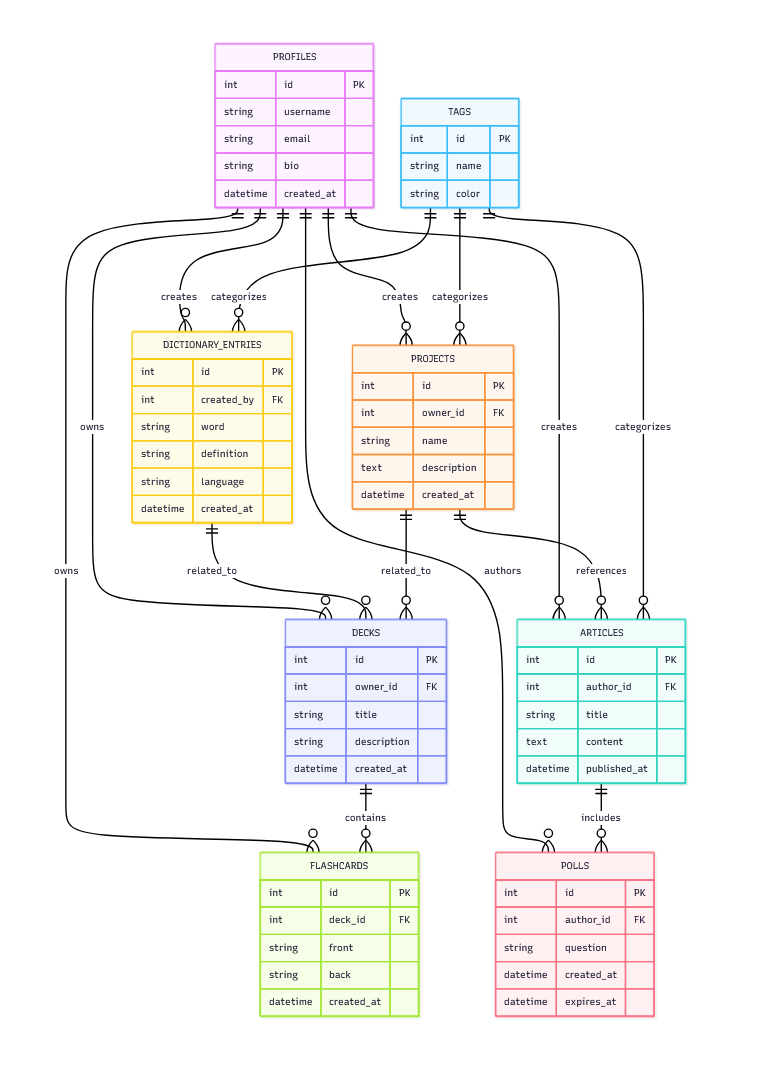
\includegraphics[width=0.92\textwidth]{pictures/general-erdiagram.png}
\caption{FutureHub системийн хялбаршуулсан ER диаграм}
\end{figure}

\subsection{Class диаграм}

\begin{figure}[H]
\centering
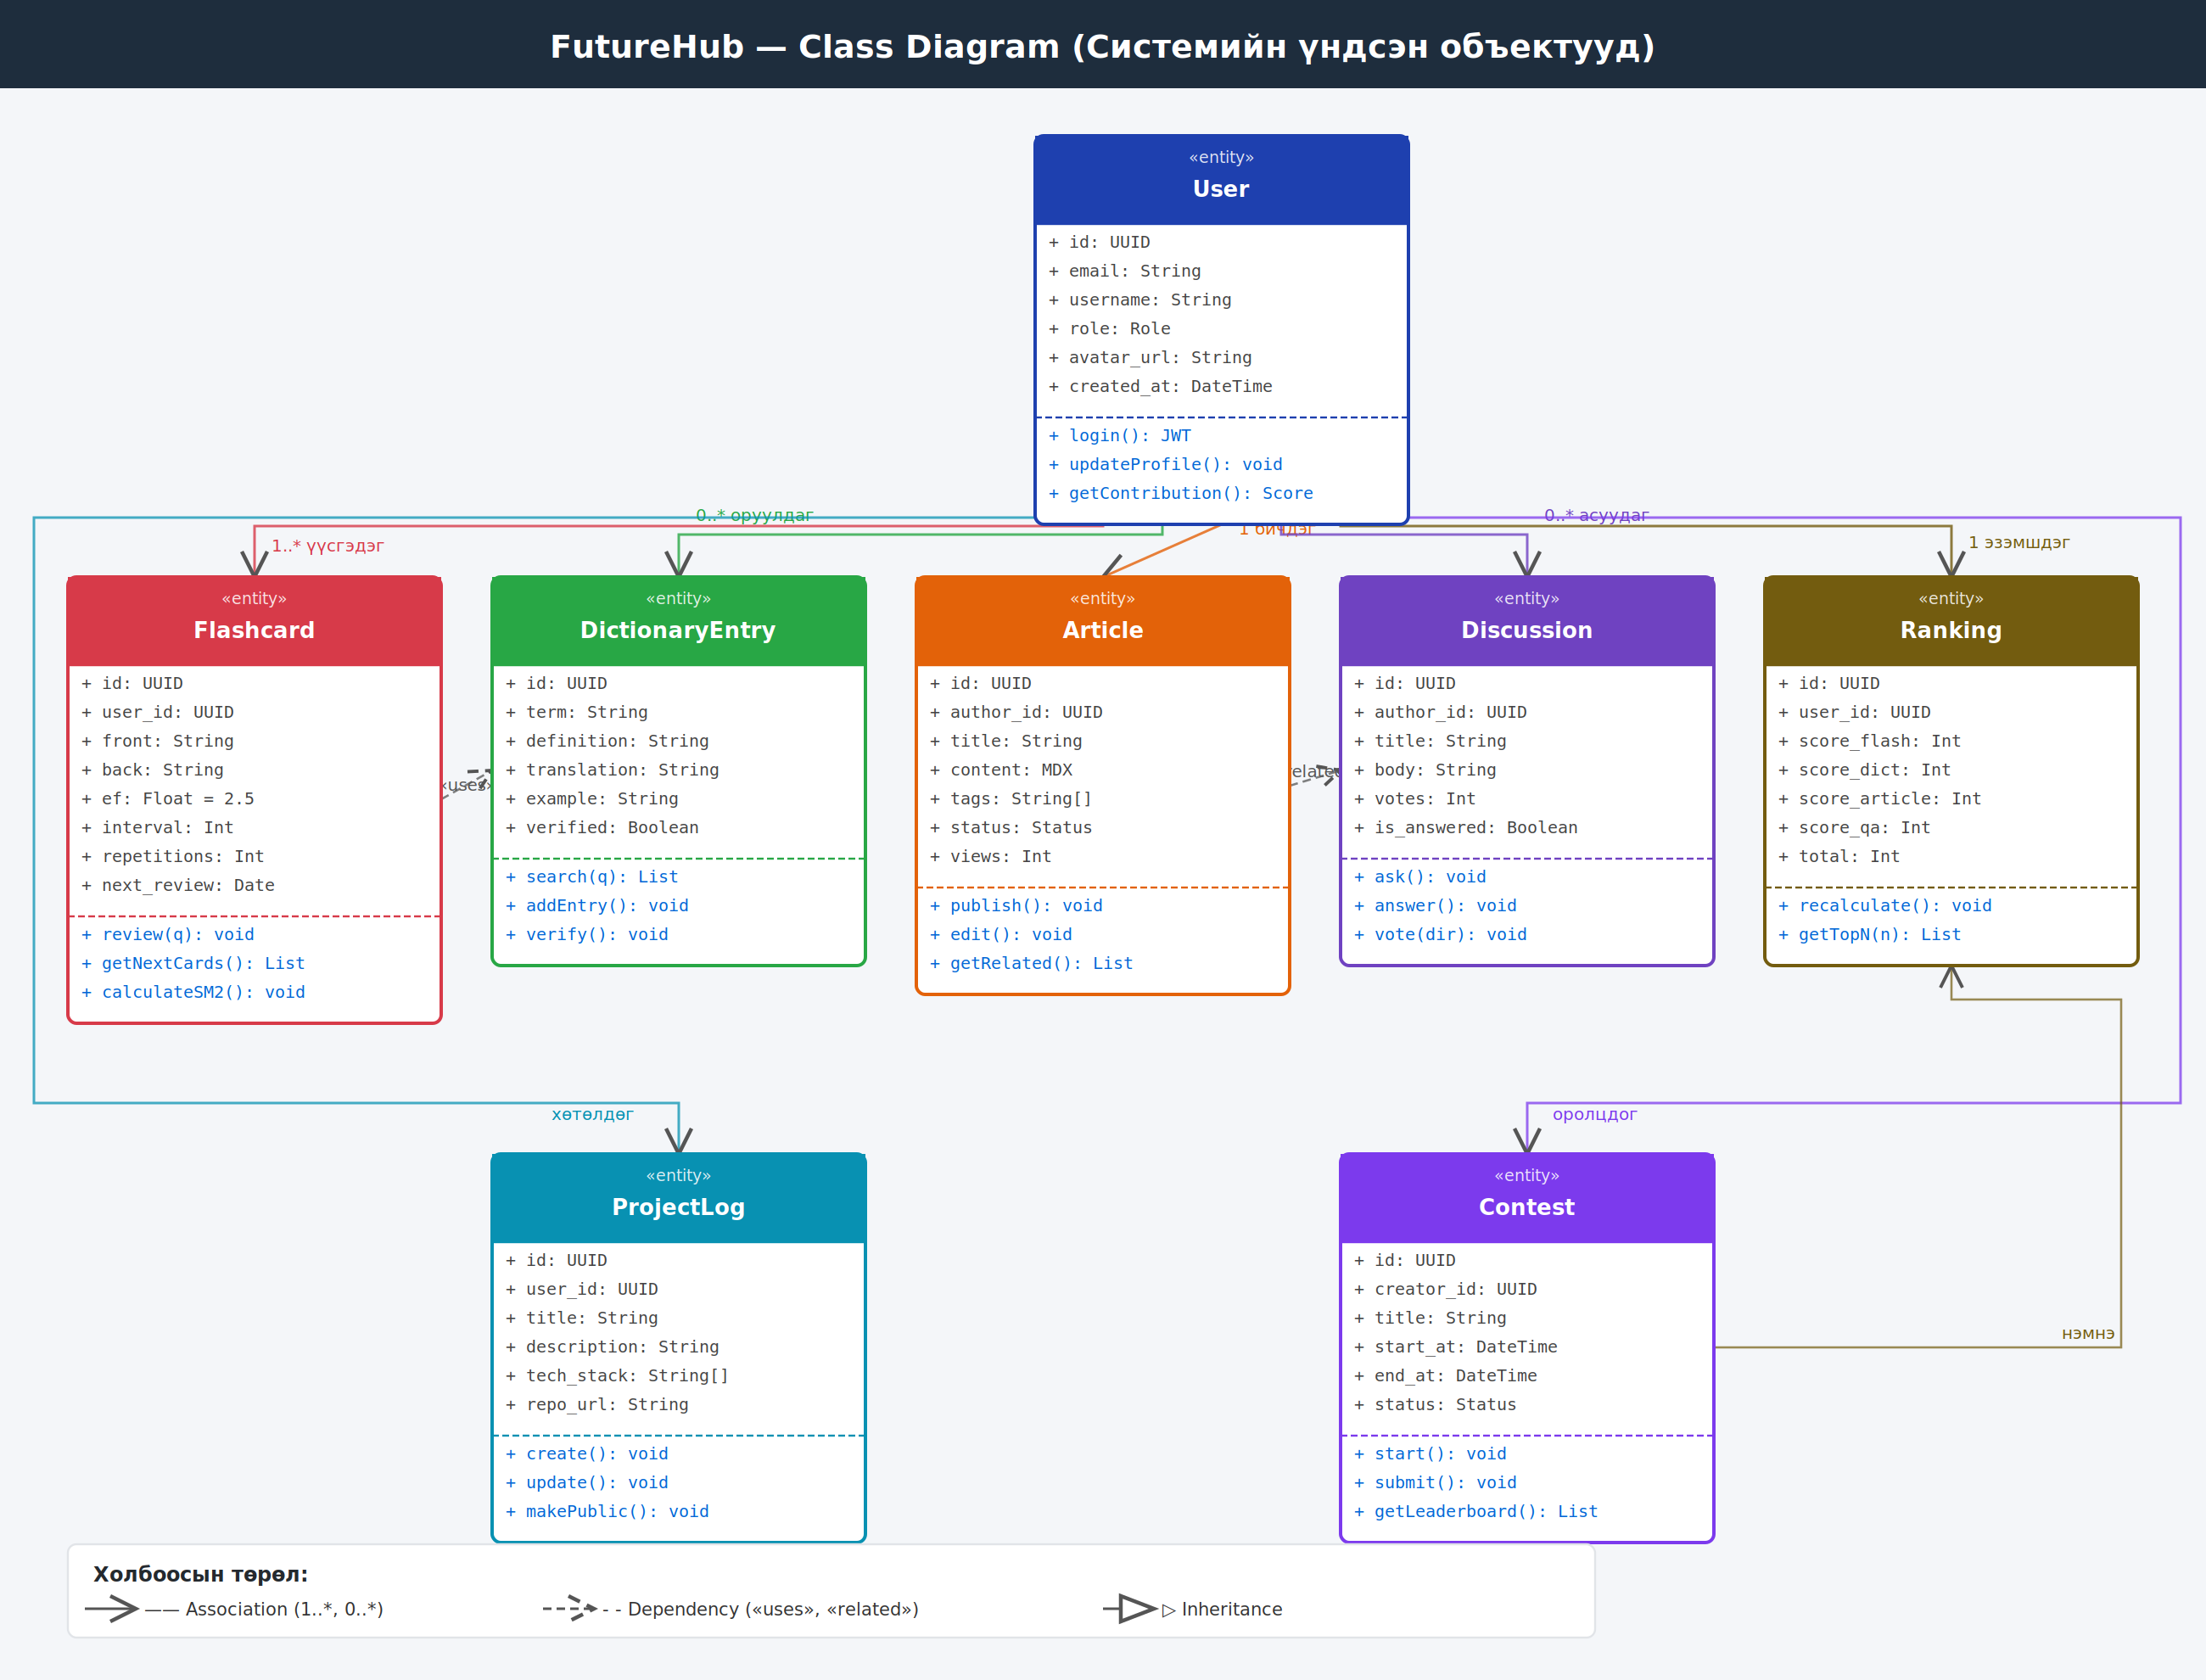
\includegraphics[width=0.92\textwidth]{pictures/futurehub_4_class.png}
\caption{FutureHub системийн Class диаграм}
\label{fig:futurehub-class}
\end{figure}

Class диаграм нь системийн өгөгдлийн объектууд болон тэдгээрийн хоорондын хамаарлыг бүтцийн түвшинд илэрхийлнэ (Зураг~\ref{fig:futurehub-class}). Диаграмд \texttt{User}, \texttt{Flashcard}, \texttt{DictionaryEntry}, \texttt{Article}, \texttt{Discussion}, \texttt{Contest}, \texttt{Ranking} зэрэг үндсэн объектууд болон эдгээрийн хоорондын хамаарлыг харуулсан. Энэ нь системийн архитектурын суурь бүтцийг тодорхойлох, хөгжүүлэлтийн явцад өгөгдлийн зохион байгуулалт ба харилцааг ойлгоход чухал үүрэгтэй болно.


%==============================================================
\section{Алгоритмын шийдлүүд}
%==============================================================



\subsection{SRS алгоритм (SM-2)}

Флашкарт давталтыг \textbf{SM-2 (SuperMemo-2)} алгоритм дээр суурилуулан хэрэгжүүлсэн. Гол параметрүүд нь $EF$ (Easiness Factor), $I_n$ (интервал), $n$ (давталтын тоо), болон $q$ (хэрэглэгчийн гүйцэтгэлийн үнэлгээ, $0 \le q \le 5$) юм.

Интервал шинэчлэх томьёо:
\[
I_1 = 1, \quad I_2 = 6, \quad I_n = I_{n-1} \cdot EF \;\;(n \ge 3)
\]

Easiness Factor-ын шинэчлэлт:
\[
EF' = EF + \bigl(0{,}1 - (5-q)\cdot(0{,}08 + (5-q)\cdot 0{,}02)\bigr), \quad EF' \ge 1{,}3
\]

Хэрэглэгчийн үнэлгээ $q < 3$ байвал давталт эхнээсээ эхэлнэ ($n \leftarrow 0$, $I \leftarrow 1$). Ийнхүү алгоритм нь хэрэглэгчийн мэдлэгийн тогтоц муу карт дээр илүү олон давтамжтай, тогтсон карт дээр үсрэнгүй интервалтай ажиллах замаар хувь хүнд тохирсон давталтын хуваарь үүсгэнэ.

\subsection{Ranking систем}

Хэрэглэгчийн хувь нэмрийн онооны ерөнхий загварыг модулиудын жинлэсэн нийлбэрээр дараах байдлаар тодорхойлов:
\[
\mathrm{Score}(u) = \sum_{i=1}^{n} w_i \cdot x_i(u)
\]

энд $x_i(u)$ нь $u$ хэрэглэгчийн $i$-р модуль дахь гүйцэтгэлийн хэмжүүр (жишээ нь: нийтэлсэн нийтлэлийн тоо, хариулсан асуултын тоо, флашкарт давтсан тоо), $w_i$ нь тухайн модулийн ач холбогдлын жин юм. Модулийн хоорондох хэмжээсийн ялгааг арилгахын тулд $x_i$ утгуудыг нормчлолтой байдлаар нэгтгэдэг:
\[
\hat{x}_i = \frac{x_i}{\max_{u'} x_i(u')}
\]

Ингэснээр аль нэг модулийн өндөр үзүүлэлттэй хэрэглэгч бусдыг \textit{дарах} нөлөөг багасгаж, хүчин зүйлүүдийн хэмжилтийн нэгжийг нэг жигд түвшинд оруулна.

\subsection{Хайлтын логик}

Нэр томьёо, нийтлэл, асуултын хайлтыг PostgreSQL-ийн \textit{full-text search} механизмыг ашиглан хэрэгжүүлсэн. Хайлтын чанарыг дараах байдлаар сайжруулсан:

\begin{itemize}
    \item \texttt{tsvector} талбарт GIN индекс үүсгэн хайлтын хурдыг оновчилсон
    \item Tag-т суурилсан шүүлтүүрийг \texttt{ts\_query}-тэй хавсран ажиллуулах
    \item Үр дүнг \texttt{ts\_rank\_cd} функцээр чухал үг-хамаарлаар эрэмбэлэх
\end{itemize}

\section{UI/UX дизайн}

UI/UX дизайны хувьд дараах зарчмуудыг баримталсан:

\begin{itemize}
    \item \textbf{Screen Flow:} хэрэглэгчийн үүрэг бүрийн гол урсгалыг зураглан гаргасан
    \item \textbf{Wireframe:} дэлгэц бүрийн бүтэц, мэдээллийн шаталсан зохион байгуулалтыг урьдчилан загварчилсан
    \item \textbf{Дизайн систем:} өнгө, typography, компонентыг дахин ашиглах загвараар нэгтгэсэн
    \item \textbf{Компонентын тогтвортой байдал:} веб болон мобайл дээр ижил үйлдлийн логик, ижил нэршлийг баримталж, платформ хооронд шилжихэд хэрэглэгчийн танин мэдэхүйн ачаалал багасахаар зохион байгуулсан
\end{itemize}

\begin{figure}[H]
\centering
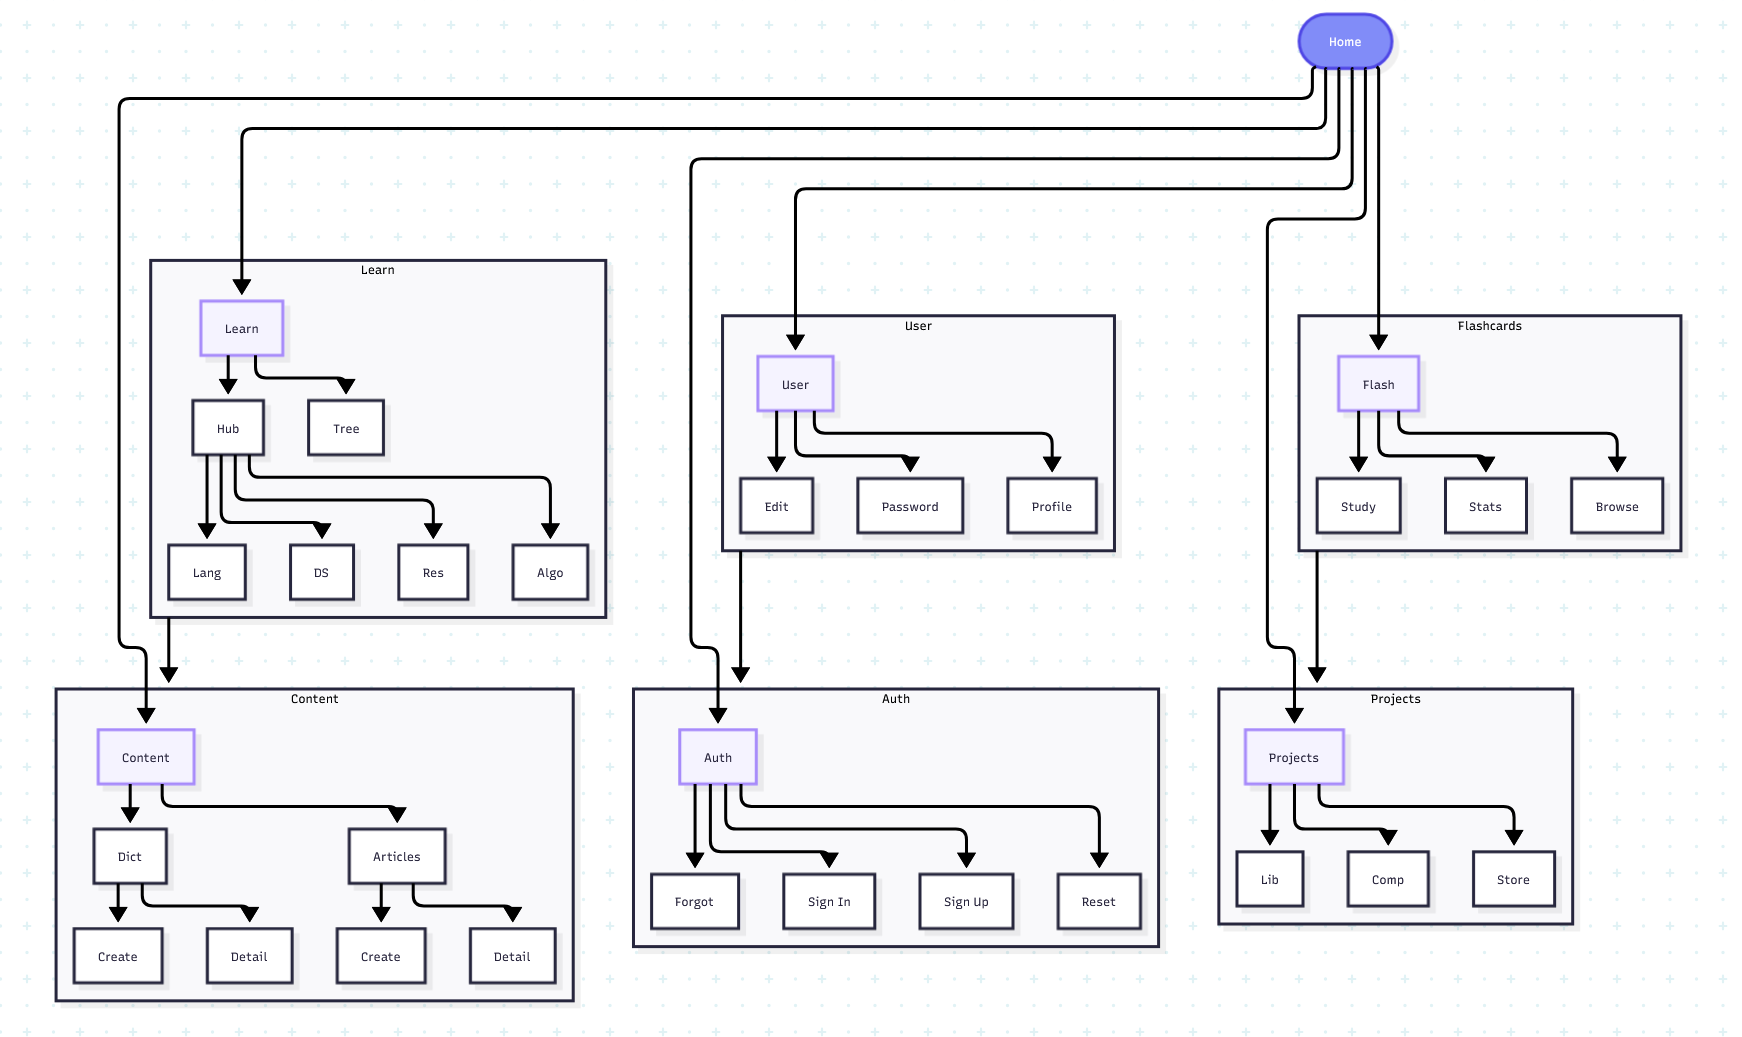
\includegraphics[width=0.98\textwidth]{pictures/display-tree.png}
\caption{FutureHub системийн дэлгэцийн загвар (Display tree)}
\label{fig:display-tree}
\end{figure}

%==============================================================
\section{Хөгжүүлэлт ба туршилтын аргачлал}
%==============================================================

\subsection{Хөгжүүлэлтийн мөчлөг}

Итератив загварын хүрээнд дараах дарааллаар хөгжүүлэлтийг гүйцэтгэсэн:

\begin{enumerate}[leftmargin=2em]
    \item \textbf{Суурь бүтэц:} authentication, navigation, layout-ийн загварууд
    \item \textbf{Core модулиуд:}  projects, dictionary, Q\&A, article
    \item \textbf{Extended модулиуд:} contest, analytics, flashcard
    \item \textbf{Нэгтгэл ба уялдаа:} ranking, profile, модуль хоорондын өгөгдлийн урсгал
    \item \textbf{Мобайл нутагшуулалт:} веб дээрх бизнес логикийг Flutter орчинд тусгах
\end{enumerate}

Git workflow-ийн хувьд \textit{feature branch} стратеги баримталж, кодын чанарыг pull request ба code review процессоор хянасан. 

\subsection{Туршилтын аргачлал}

Туршилтыг гурван түвшинд зохион байгуулсан:

\begin{itemize}
    \item \textbf{Unit test:} тусдаа функц, алгоритмын (SRS-ийн интервал бодолт, ranking-ийн оноо тооцоолол гэх мэт) логикийн зөв ажиллагааг шалгах
    \item \textbf{Integration test:} модуль хоорондын API дуудлага, өгөгдлийн сангийн харилцан үйлчлэлийг баталгаажуулах
    \item \textbf{UAT (User Acceptance Testing):} бодит хэрэглэгчдийн сценари дээр суурилан хэрэглэгчийн туршлагын түвшинд баталгаажуулах
\end{itemize}

\subsection{Үнэлгээний шалгуур}

Системийн амжилтыг дараах шалгуур үзүүлэлтүүдээр үнэлнэ:

\begin{itemize}[leftmargin=2em]
    \item Системийн найдвартай ажиллагаа --- үндсэн урсгалууд алдаагүй ажиллах байдал
    \item OCR-ийн нарийвчлал --- танилтын зөв хувь (accuracy)
    \item Ранкингийн логикийн зөв байдал --- хэрэглэгчийн үйлдэл ба оноо хоорондын уялдаа
    \item SRS давталтын үнэн зөв шинэчлэлт --- интервал, $EF$-ийн тооцооллын алдаагүй байдал
    \item API хариуны гүйцэтгэл --- дундаж хариу өгөх хугацаа, ачаалал даах чадвар
\end{itemize}